\chapter{k-copy Randomised Benchmarking}
\minitoc
%
Building on the general twirling formalism and noise models of
Chapter~\ref{chap:background}, this chapter introduces \emph{$k$-copy
randomised benchmarking}: an RB protocol in which identical single-qubit
Clifford sequences are applied in parallel across multiple qubits, and
pairwise measurement correlations are retained rather than averaged away.
We derive the resulting population dynamics for the common-noise model of
Section~\ref{sec:common_noise}, and present experimental demonstrations on
a trapped-ion processor, including isolation of correlated versus local
error, a parity-based confirmation of the underlying symmetric-subspace
occupation, a controlled noise-injection scan, and scaling to an eight-ion
register.

% ==========================================================================
\section{Existing approaches to correlated-noise characterisation}
\label{sec:existing_approaches}
% literature review of existing approaches to correlated-noise characterisation

\todo{Define spatial correlations (do in theory section?)}

Existing approaches to correlated-noise characterisation span a trade-off
between expressiveness and scalability. Tomographic and noise-learning
techniques can reconstruct detailed structure in the error channel, but
their cost grows rapidly with system
size~\cite{rudinger_experimental_2021, harper_efficient_2020,
harper_learning_2023, nielsen_efficient_2021}. Random circuit methods,
including randomised benchmarking, are substantially more scalable, but
typically compress the action of noise into a small number of averaged
parameters~\cite{sarovar_detecting_2020, mckay_correlated_2020,
erhard_characterizing_2019, gambetta_characterization_2012,
magesan_scalable_2011}.

A related RB protocol, termed ``Correlated RB''~\cite{mckay_correlated_2020}
(itself built on ``Simultaneous RB''~\cite{gambetta_characterization_2012}),
uses \emph{independent} local twirling of multiple system copies to estimate
the distance of the measured channel from a product (uncorrelated) channel.
This differs fundamentally from the \emph{identical}-sequence twirling
strategy developed in Chapter~\ref{chap:results}: independent local
twirling averages away exactly the symmetry information that identical
twirling preserves.

A complementary source of inspiration comes from correlation spectroscopy
and decoherence-free-subspace techniques, where common-mode noise is
revealed through its action on collective and differential degrees of
freedom~\cite{clements_lifetime-limited_2020}. In such settings, symmetry is
not merely a simplifying assumption: it is the very mechanism that separates
common fluctuations from local noise. This observation --- that enforcing a
symmetry can make correlated dynamics directly visible without
reconstructing the full many-qubit channel --- is the guiding idea carried
into Chapter~\ref{chap:results}, where it is realised concretely as
\emph{$k$-copy randomised benchmarking}.

\begin{table}
    \begin{center}
    \begin{tabular}{|c|l|}
        \hline
        Parameter & Value \\
        \hline
        729-nm laser power & 1000~\unit{\uW}\\
        \hline
    \end{tabular}
    \end{center}
    \caption{
        \todo{Summary table of other methods}
        }
    \label{tab:state_prep_parameters}
\end{table}

\todo{Add a comparative summary table at the end of this section (methods
$\times$ \{scalability, expressiveness, assumptions, experimental
requirements\}) contrasting tomography, Simultaneous RB, Correlated RB,
cycle benchmarking, and $k$-copy RB. This would give the reader a single
reference point before moving into Chapter~\ref{chap:results}.}

% ==========================================================================
\section{The $k$-copy RB protocol}
\label{sec:protocol}
\begin{figure}
    \begin{center}
    \noindent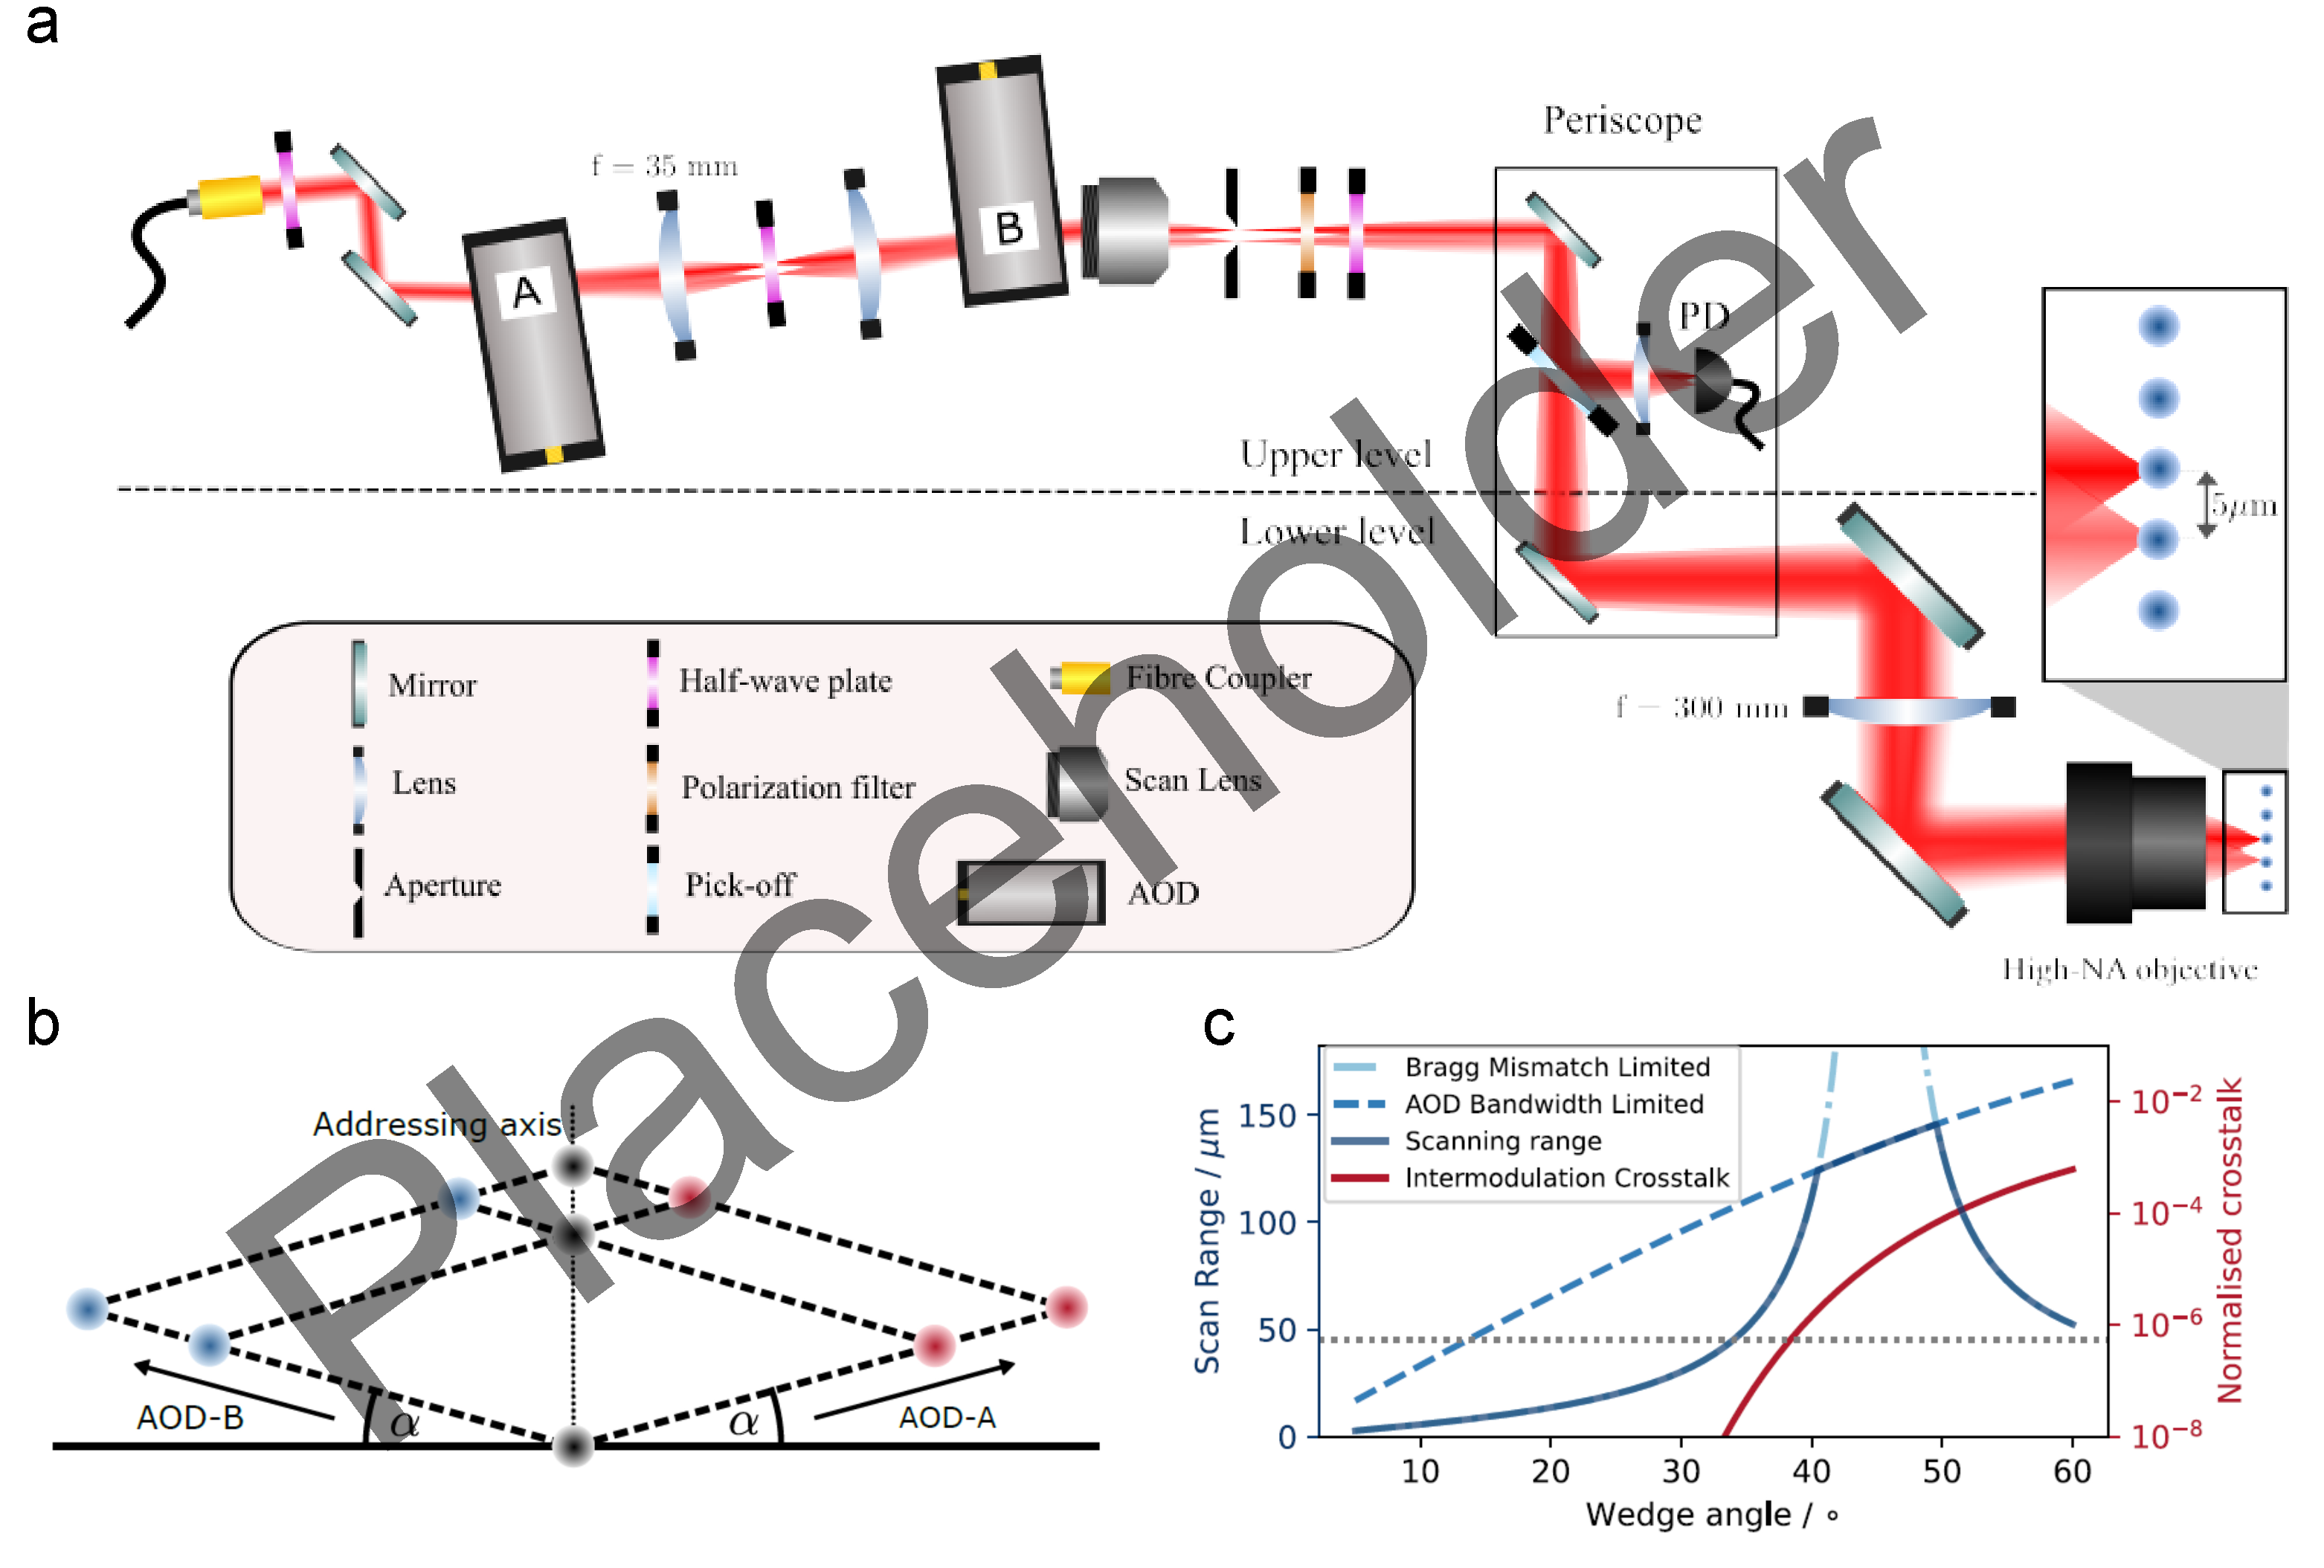
\includegraphics[width=\linewidth]{figures/pdf_figure/ch2/AOD_setup.pdf
        }
    \end{center}
    \caption{
        \todo{Circuit diagram for $k$-copy RB.}
        }
    \label{fig:AOD}
\end{figure}

We introduce a symmetry-based viewpoint into randomised benchmarking through
$k$-copy RB. In $k$-copy RB, the same single-qubit Clifford sequence is
applied in parallel to multiple qubits. This diagonal Clifford twirl
preserves symmetry sectors that are invisible to standard single-qubit RB
(Section~\ref{sec:standard_rb}) but become accessible through pairwise
measurement outcomes. For two qubits, this symmetry separates local
single-qubit decay from collective two-copy dynamics.

Concretely, the protocol applies a standard single-qubit Clifford RB
sequence~\cite{dankert_exact_2009, magesan_scalable_2011} simultaneously to
multiple qubits, with the \emph{same} randomly sampled Clifford applied to
every qubit at each step. For each sequence length $M$, $r$ random Clifford
sequences are generated and each appended with its inverting Clifford, as in
conventional RB, with each sequence repeated $s$ times. As in standard RB,
the target computational state is randomised between $\ket{0}$ and $\ket{1}$
per sequence to reduce sensitivity to SPAM asymmetries
(Section~\ref{sec:background_spam}).

\todo{(a) Circuit diagram for $k$-qubit parallel Clifford RB. (b)
Schematic single-qubit final states before measurement, sequence by
sequence. (c) Bloch-sphere ensembles for correlated vs.\ uncorrelated qubit
pairs.}{The $k$-copy protocol: identical parallel single-qubit Clifford RB
sequences applied across $k$ qubits (adapted from manuscript Fig.~1).
\todo{Redraw for thesis; consider splitting panel (c) out into its own
figure with expanded discussion of the joint-angle-distribution picture
(see note at end of Section~\ref{sec:protocol_analysis}).}}

The distinguishing feature of $k$-copy RB relative to standard or
Simultaneous RB (Section~\ref{sec:existing_approaches}) is the combination
of identical Clifford sequences with shot-resolved post-processing of
\emph{correlated} outcomes. For each qubit pair $(i,j)$, every shot is
assigned to one of four outcomes, $P_{SS}^{(i,j)}$, $P_{SF}^{(i,j)}$,
$P_{FS}^{(i,j)}$, or $P_{FF}^{(i,j)}$, where $S$ and $F$ denote success and
failure relative to the sequence-dependent target outcome. Standard
single-qubit RB averages this data into independent survival probabilities
(Eq.~\eqref{eqn:1q_rb_decay}), collapsing the dynamics to a single
exponential decay. By retaining pairwise correlations between successes and
failures instead, $k$-copy RB distinguishes shared, sequence-dependent
deviations from independent local decay. For a register of $k$ qubits, a
single shot record simultaneously contains outcomes for all $k(k-1)/2$
pairs, so extracting pairwise correlations requires only additional
classical post-processing and no extra trials on the quantum register
(this scaling property is used explicitly in Section~\ref{sec:scaling}).

Formally, applying identical Cliffords across $k$ qubits implements the
twirled representation of the single-qubit Clifford group, $Cl^{\otimes k}$.
For two qubits, this is exactly the representation analysed generally in
Section~\ref{sec:two_copy_cliff}: the twirl decomposes the two-qubit
Liouville space into the symmetry-informed subspaces of
Table~\ref{table:irreps}. The remainder of this chapter uses that
decomposition, together with the common-noise model of
Section~\ref{sec:common_noise}, to derive concrete, fittable predictions for
the correlated populations measured in a $k$-copy RB experiment.

\todo{Add a short worked numerical example here (e.g.\ a simulated
two-qubit trace showing $P_{SS}, P_{SF}, P_{FS}, P_{FF}$ for a chosen
$\{\varepsilon_L, \varepsilon_R, \varepsilon_{\mathrm{corr}}\}$) to make the
abstract shot-bookkeeping description concrete before moving to the
analytic derivation.}

\subsection{Illustrating correlated vs.\ uncorrelated signatures}
\label{sec:protocol_analysis}
%Figure 1 from paper
\begin{figure}
    \begin{center}
    \noindent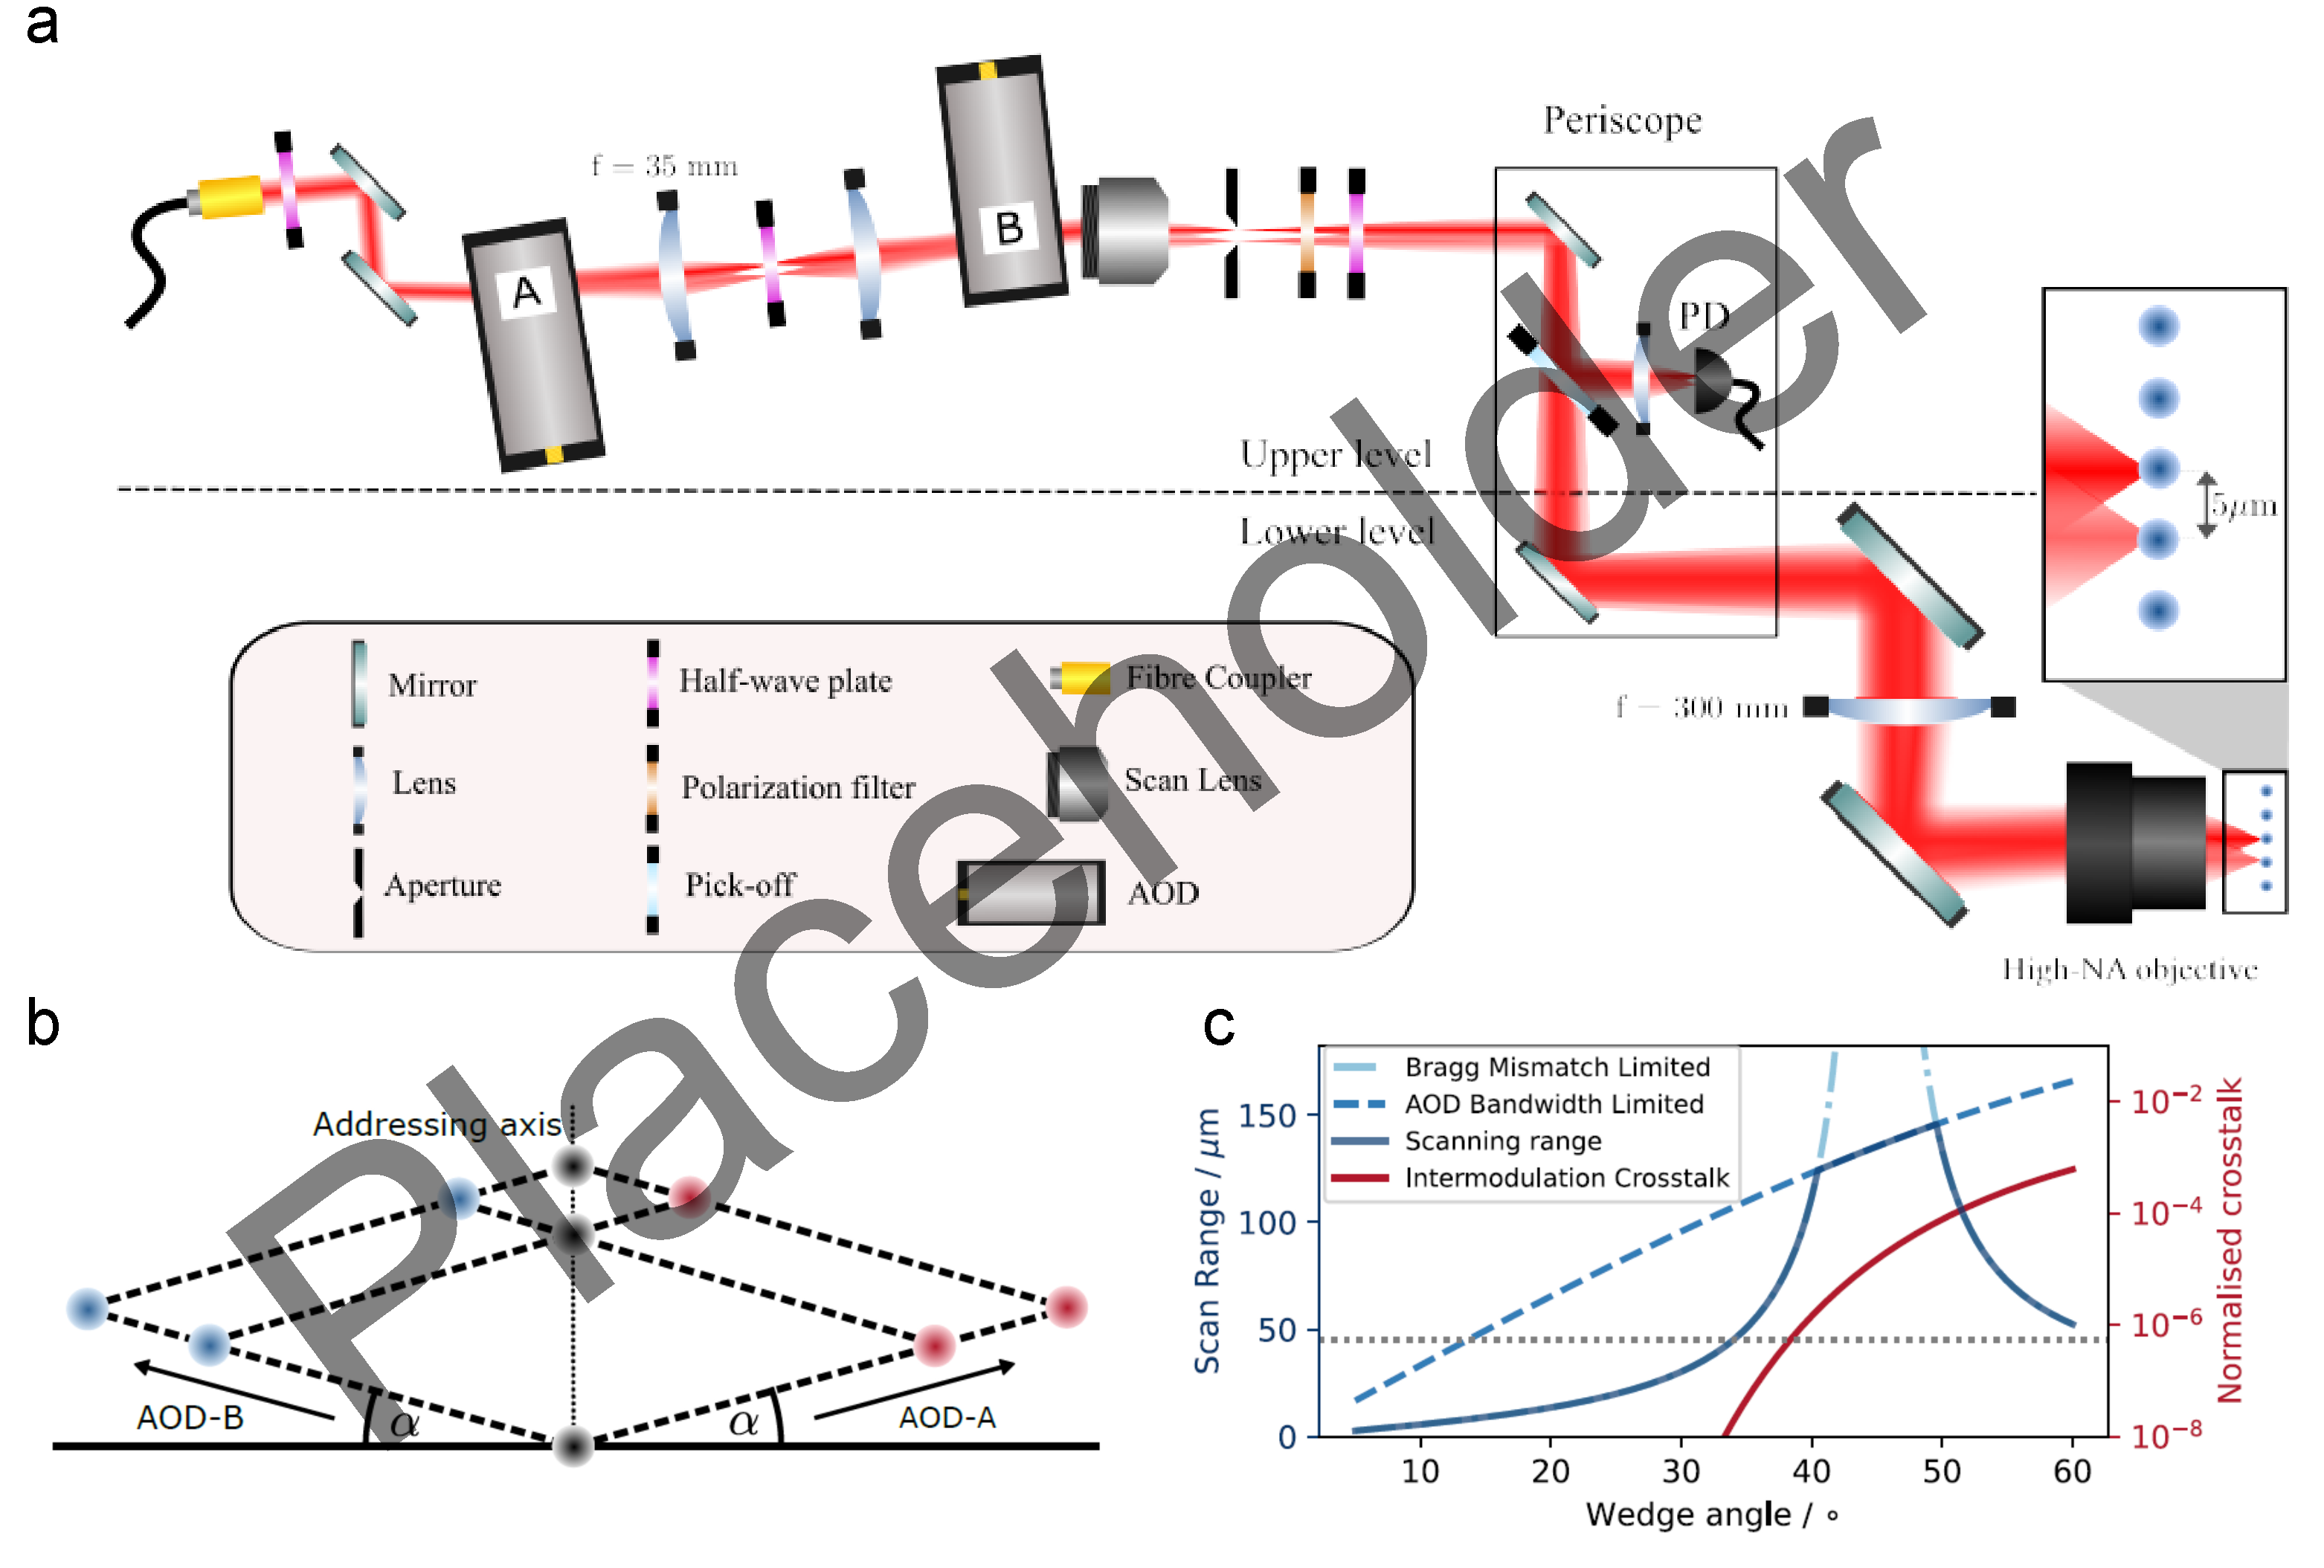
\includegraphics[width=\linewidth]{figures/pdf_figure/ch2/AOD_setup.pdf
        }
    \end{center}
    \caption{
        \todo{Bloch sphere schematic of corr vs uncorr noise. Include schematic of ion chain prev fig 1c.}
        }
    \label{fig:AOD}
\end{figure}

The distinction between correlated and uncorrelated noise is illustrated
schematically by considering a register in which qubits $i=3$ and $i=4$ are
dominated by a common rotation error while other qubits are dominated by
independent noise. All qubits can exhibit identical single-qubit RB error
rates (i.e.\ an identical depolarised Bloch vector under standard RB), while
possessing entirely different pairwise correlation structure: independent
noise produces uncorrelated sequence-to-sequence deviations, whereas common
noise produces shared deviations between qubits acted on by the same random
Clifford sequence. The identical-sequence condition is therefore essential
to the protocol: it preserves exactly the symmetry information that would be
averaged away under independently sampled local Clifford sequences (as in
Simultaneous/Correlated RB, Section~\ref{sec:existing_approaches}).

\todo{This is currently a qualitative, schematic argument (matching the
level of detail in the PRL). A thesis chapter could usefully add the
joint-angle-distribution analysis that was drafted but cut from the
manuscript: uncorrelated noise exponentially suppresses higher-weight error
terms $p_w = \prod_i p_i$ relative to single-qubit rates, whereas correlated
noise violates this independence assumption and can scale linearly with
weight $w$ in the worst case, with consequences for QEC thresholds assuming
independent errors ($p_t \propto \theta_i^2\theta_j^2$). This connects
naturally to the $>2$-qubit scaling results in
Section~\ref{sec:scaling}.}

% ==========================================================================
\section{Analytic predictions for common noise}
\label{sec:analytic_predictions}

\subsection{Correlated population decay}

\begin{figure}
    \begin{center}
    \noindent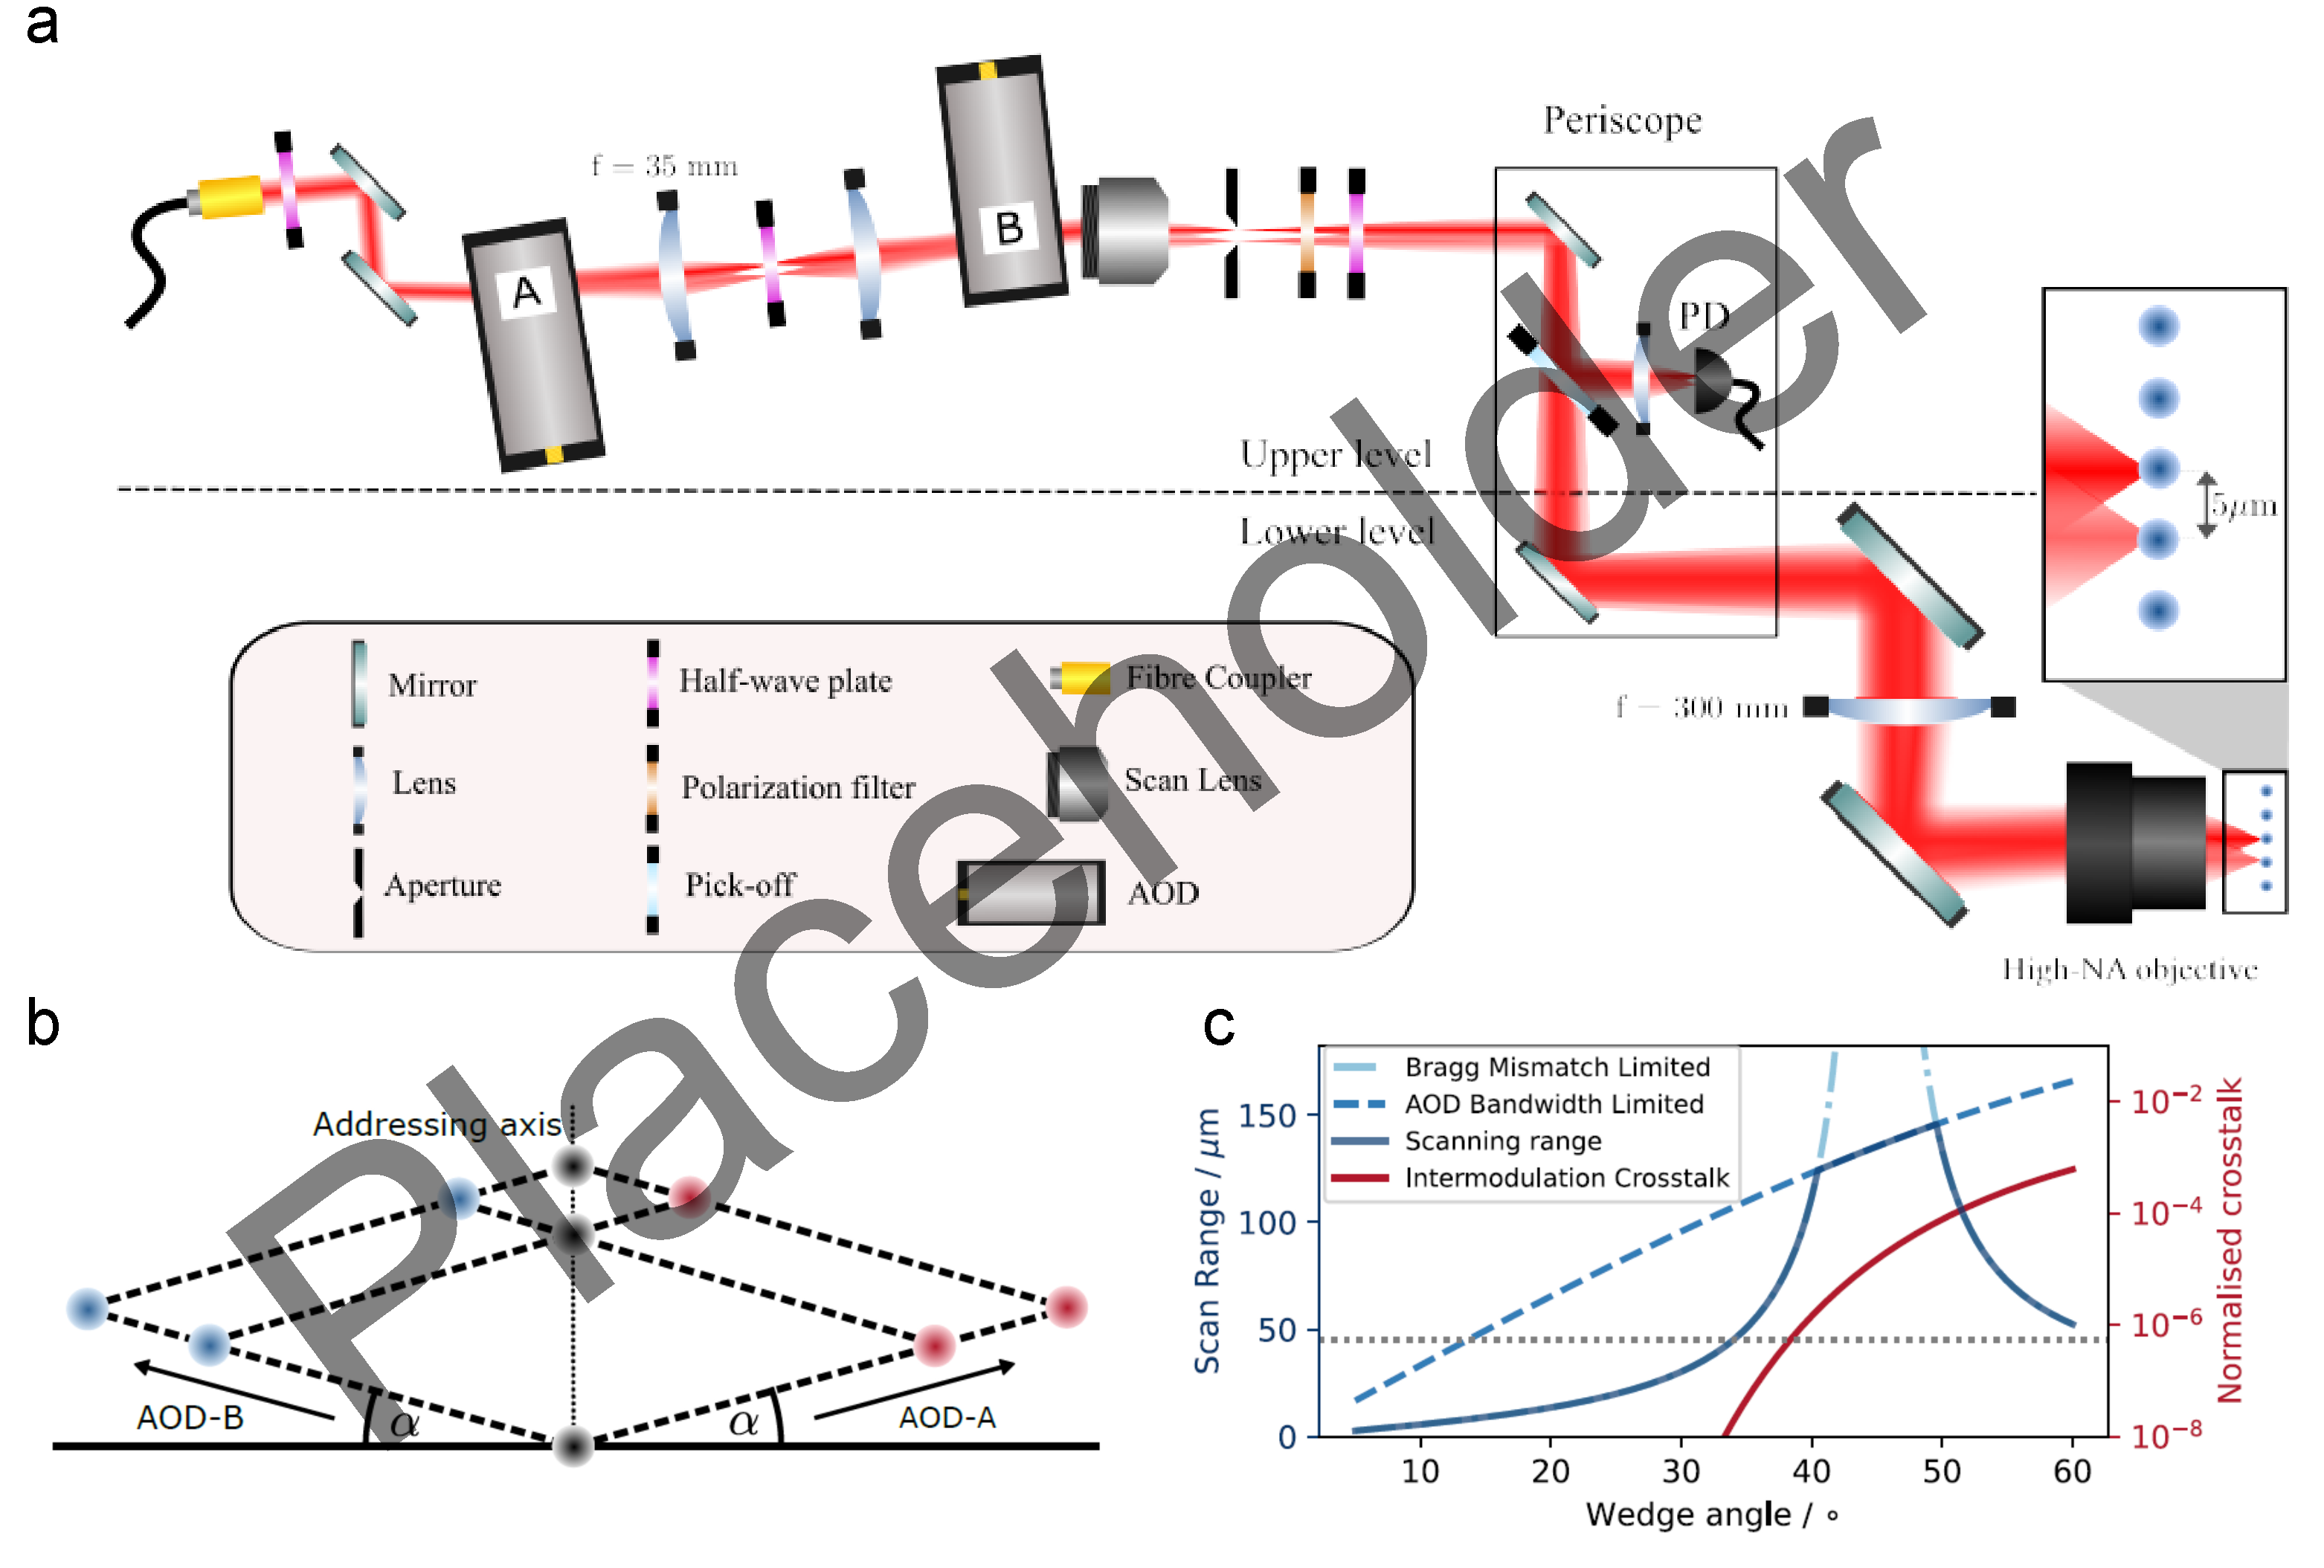
\includegraphics[width=\linewidth]{figures/pdf_figure/ch2/AOD_setup.pdf
        }
    \end{center}
    \caption{
        \todo{Numerical simulation of intermediate asymptotes measured in Z basis.}
        }
    \label{fig:AOD}
\end{figure}
Using the block-diagonal Liouville structure of
Eq.~\eqref{eqn:block_diagonal} and the scalar decay rates it implies, the
probability of both qubits successfully returning to their initial state
after $m$ Cliffords, for a general error channel diagonal in the irrep
basis of Table~\ref{table:irreps}, is
\begin{equation}
    \mathcal{P}_{SS} = \frac{1}{4} + \frac{1}{4}\left(\alpha_L^m + \alpha_R^m\right)
    + \frac{1}{6}\alpha_{dt}^m + \frac{1}{12}\alpha_{tr}^m,
    \label{eqn:decay}
\end{equation}
with corresponding expressions for $\mathcal{P}_{SF}$, $\mathcal{P}_{FS}$,
and $\mathcal{P}_{FF}$ following the same structure with sign changes on the
$\alpha_L^m, \alpha_R^m$ and $\alpha_{dt}^m, \alpha_{tr}^m$ terms
respectively.

Combining the local depolarising channel
(Eq.~\eqref{eqn:local_depol_liouville}) with the twirled common-noise
channel (Section~\ref{sec:common_noise}) gives, to first order, the sector
decay rates
\begin{align}
    \alpha_L &= 1-\varepsilon_L-\varepsilon_\mathrm{corr}, &
    \alpha_R &= 1-\varepsilon_R-\varepsilon_\mathrm{corr}, \\
    \alpha_{tr} &= 1 - \varepsilon_L- \varepsilon_R, &
    \alpha_{dt} &= 1 - \varepsilon_L- \varepsilon_R - 3\varepsilon_\mathrm{corr},
    \label{eqn:bases}
\end{align}
where $\varepsilon_{\mathrm{corr}}$ is defined by Eq.~\eqref{eqn:e_corr}.
Because the symmetric trace sector is exactly invariant under common
rotation noise ($\alpha_{tr}=1$ when $\varepsilon_L=\varepsilon_R=0$),
Eq.~\eqref{eqn:decay} predicts an intermediate asymptote,
$\mathcal{P}_{SS}|_{m\to\infty} = 1/3$, distinct from the fully depolarised
asymptote $\mathcal{P}_{SS}|_{m\to\infty} = 1/4$ reached once any finite
local error rate is present. This intermediate asymptote is the central
experimental signature of correlated noise exploited throughout this
chapter, and corresponds to the two-qubit state
\begin{equation}
    \rho_{sym} = \frac{1}{3}\left(\ket{00}\bra{00} + \ket{11}\bra{11}
    + \ket{\Psi^+}\bra{\Psi^+}\right),
    \label{eqn:bell}
\end{equation}
where $\ket{\Psi^+} = \tfrac{1}{\sqrt2}(\ket{01}+\ket{10})$ is a Bell state.
The presence of this Bell-state component reflects residual coherence
induced between the two qubits by the shared rotation error, and motivates
the independent, coherence-sensitive probe developed in
Section~\ref{sec:parity}.

\todo{Insert the full derivation connecting Eq.~\eqref{eqn:decay} to the
vectorised-state inner product $\mathcal{P}_{L,R} = \langle\langle L,R|
\Lambda_T^m|00\rangle\rangle$ and the explicit transfer matrices, rather
than quoting the result (this is worked in the manuscript SM and can be
reproduced here in full for thesis completeness, including the
$\mathcal{P}_{0,1}, \mathcal{P}_{1,0}, \mathcal{P}_{1,1}$ companion
expressions).}

\subsection{Parity contrast: an independent probe of coherence}
\label{sec:parity}
\begin{figure}
    \begin{center}
    \noindent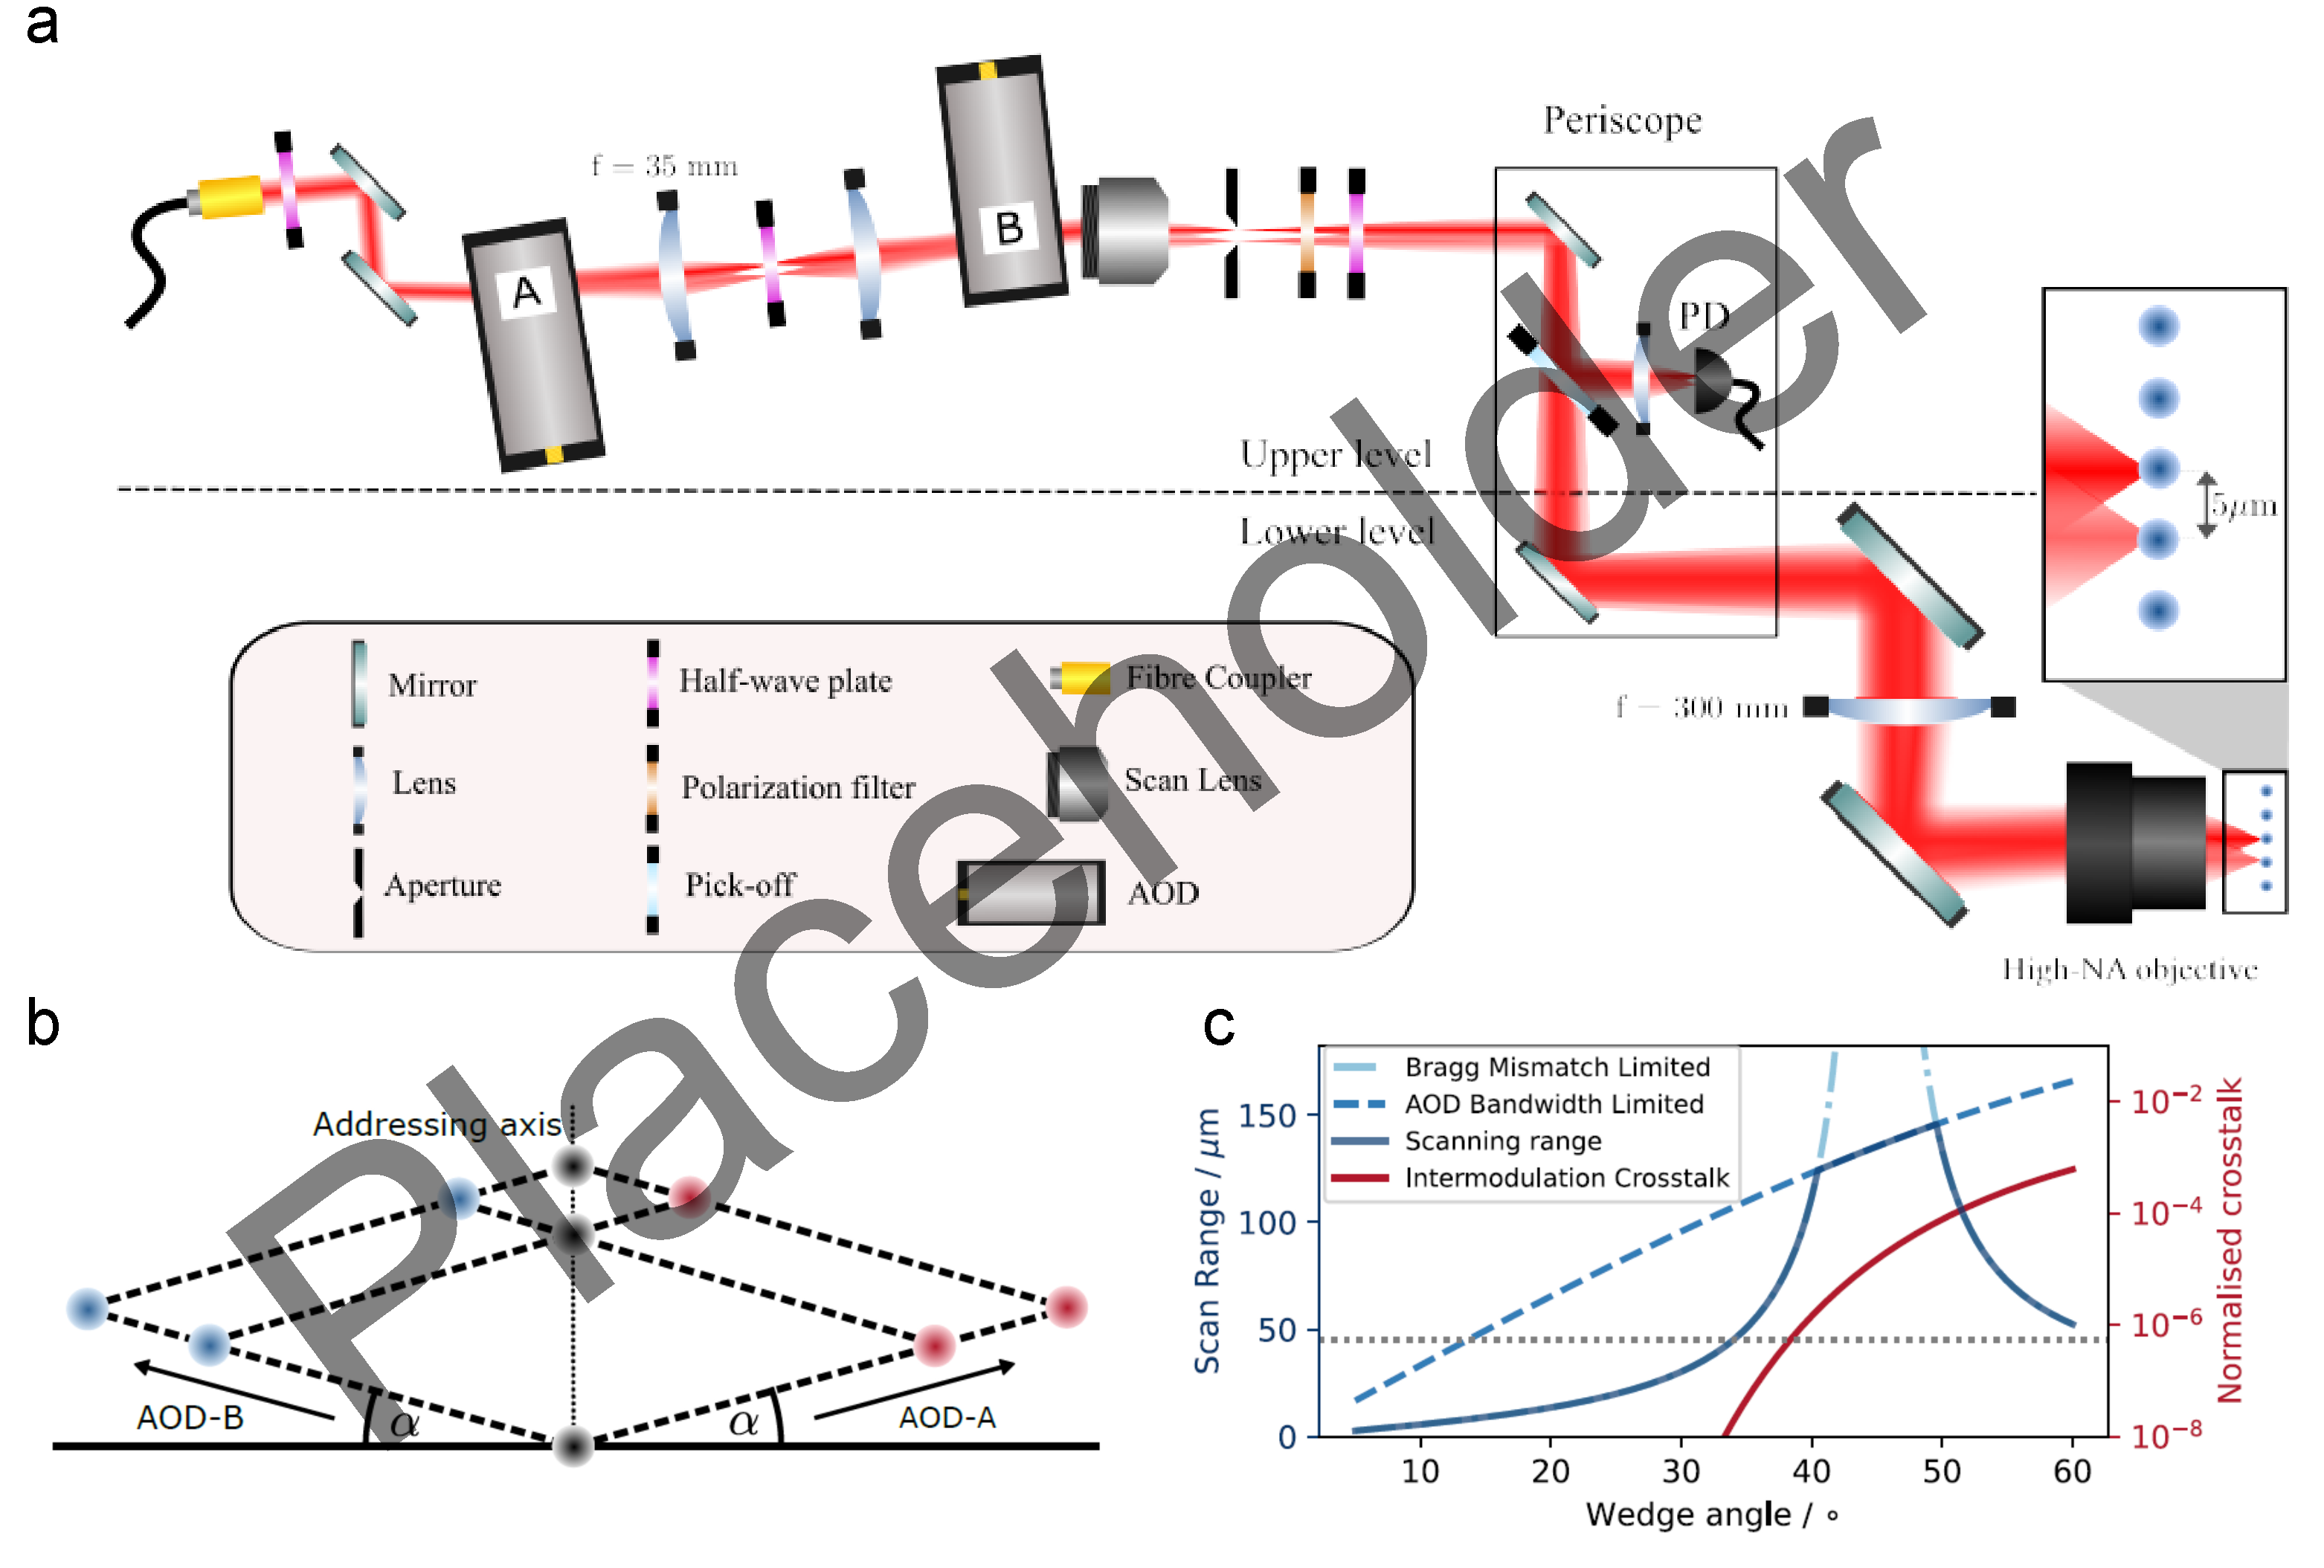
\includegraphics[width=\linewidth]{figures/pdf_figure/ch2/AOD_setup.pdf
        }
    \end{center}
    \caption{
        \todo{circuit diagram for parity measurement. Could there also be a nice schematic of the Bloch sphere picture of the differential rotation?}
        }
    \label{fig:AOD}
\end{figure}

Population decays alone indicate an intermediate asymptote; a parity-based
measurement independently verifies that this asymptote corresponds
specifically to occupation of the symmetric trace sector, by directly
probing the residual coherence $\ket{01}\bra{10}$ built up between the two
qubits. Differential rotations of the form $\hat R_{+\phi}(\pi/2) \otimes
\hat R_{-\phi}(\pi/2)$, with rotation axis $\hat\sigma_\phi$ in the
$XY$-plane, are applied prior to measurement, and the contrast of the
resulting fringe (as $\phi$ is varied) is extracted. This contrast has the
predicted dependence
\begin{equation}
    \mathcal{C} = \frac{1}{3}\left(\alpha_{tr}^m - \alpha_{dt}^m\right),
    \label{eqn:parity}
\end{equation}
with a maximum value $\mathcal{C}_{\max} = 1/3$, reached in the same regime
in which the population asymptote of Eq.~\eqref{eqn:decay} sits at $1/3$.
Equations~\eqref{eqn:decay} and~\eqref{eqn:parity} may be combined to
isolate the individual sector decay rates $\alpha_{tr}$ and $\alpha_{dt}$ as
single exponentials, rather than fitting the multi-exponential population
decay directly.

\todo{Reproduce the full parity-contrast derivation from the manuscript SM
(App.~``Parity analysis''): the transfer-matrix expression $\Pi(\phi) =
\langle\langle \pi|\Lambda_\Pi(\phi)\Lambda_T^m|00\rangle\rangle =
\mathcal{C}\cos(2\phi)$, the Bloch-sphere-averaging argument giving
$\mathcal{C}_{\max}=1/3$, and the isolation identities $\Pi_Z - C =
\alpha_{dt}^m$, $\Pi_Z + 2C = \alpha_{tr}^m$ using the computational parity
$\Pi_Z = \mathcal{P}_{0,0}+\mathcal{P}_{1,1}-\mathcal{P}_{0,1}-\mathcal{P}_{1,0}$.
This is a good candidate for a fully worked thesis subsection given its
role in confirming the central experimental claim.}

\subsection{Isolating sectors via initial-state choice}
\begin{figure}
    \begin{center}
    \noindent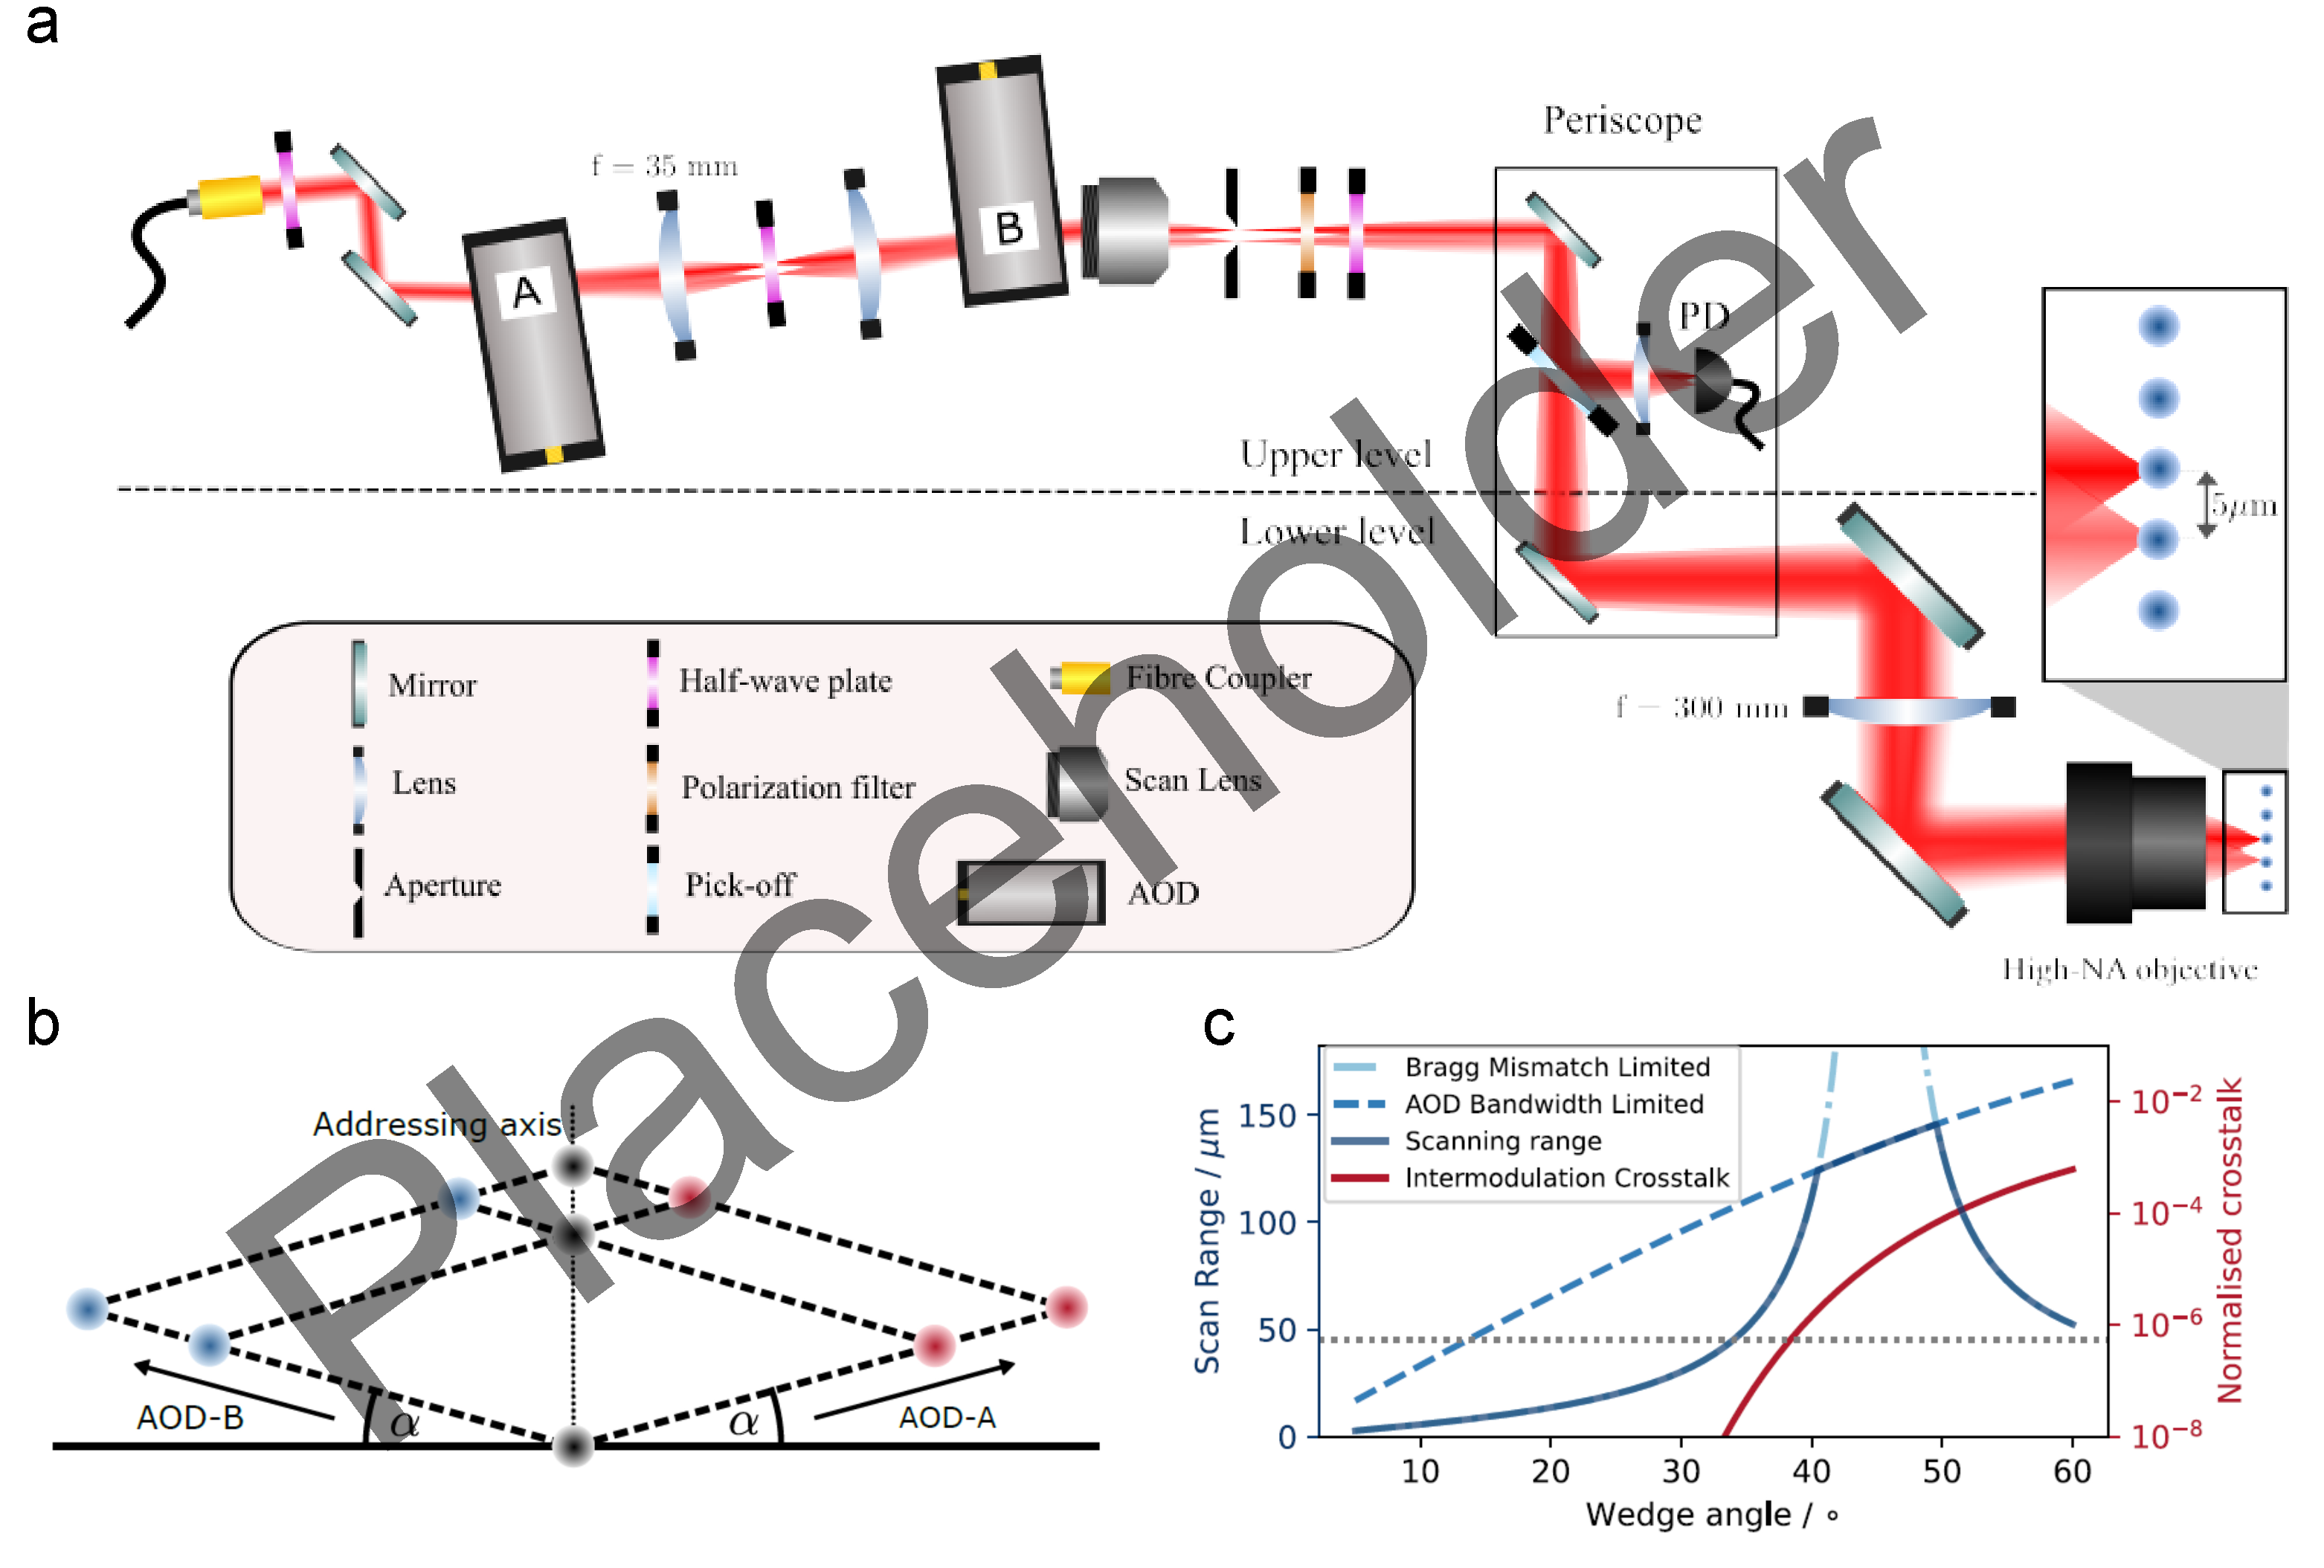
\includegraphics[width=\linewidth]{figures/pdf_figure/ch2/AOD_setup.pdf
        }
    \end{center}
    \caption{
        \todo{Block diagonal Liouville structure of the two-copy Clifford twirl, showing the sub-representations and their associated decay rates.}
        }
    \label{fig:AOD}
\end{figure}

Beyond parity measurements, the sector decomposition of
Table~\ref{table:irreps} suggests that preparing initial states with
overlap on only a subset of sub-representations can isolate individual
decay constants directly, without needing to fit multi-exponential curves.
For example, preparing the singlet state $\ket{\Psi^-} =
\tfrac{1}{\sqrt2}(\ket{01}-\ket{10})$ gives a density matrix with overlap
only on the identity and symmetric-trace sub-representations, so that the
correlated populations decay as a single exponential in $\alpha_{tr}$ alone,
insensitive to $\varepsilon_{\mathrm{corr}}$.

\todo{This subsection is included as a brief pointer to a technique
discussed only in outline in the manuscript SM (by analogy with
\emph{character RB}~\cite{helsen_new_2019}). Expand into a full worked
treatment if this state-engineering approach is pursued experimentally;
otherwise keep as a short ``future extensions'' note and cross-reference
from the Outlook (Section~\ref{sec:outlook}).}

\subsection{Scaling to $k>2$ qubits}
\begin{figure}
    \begin{center}
    \noindent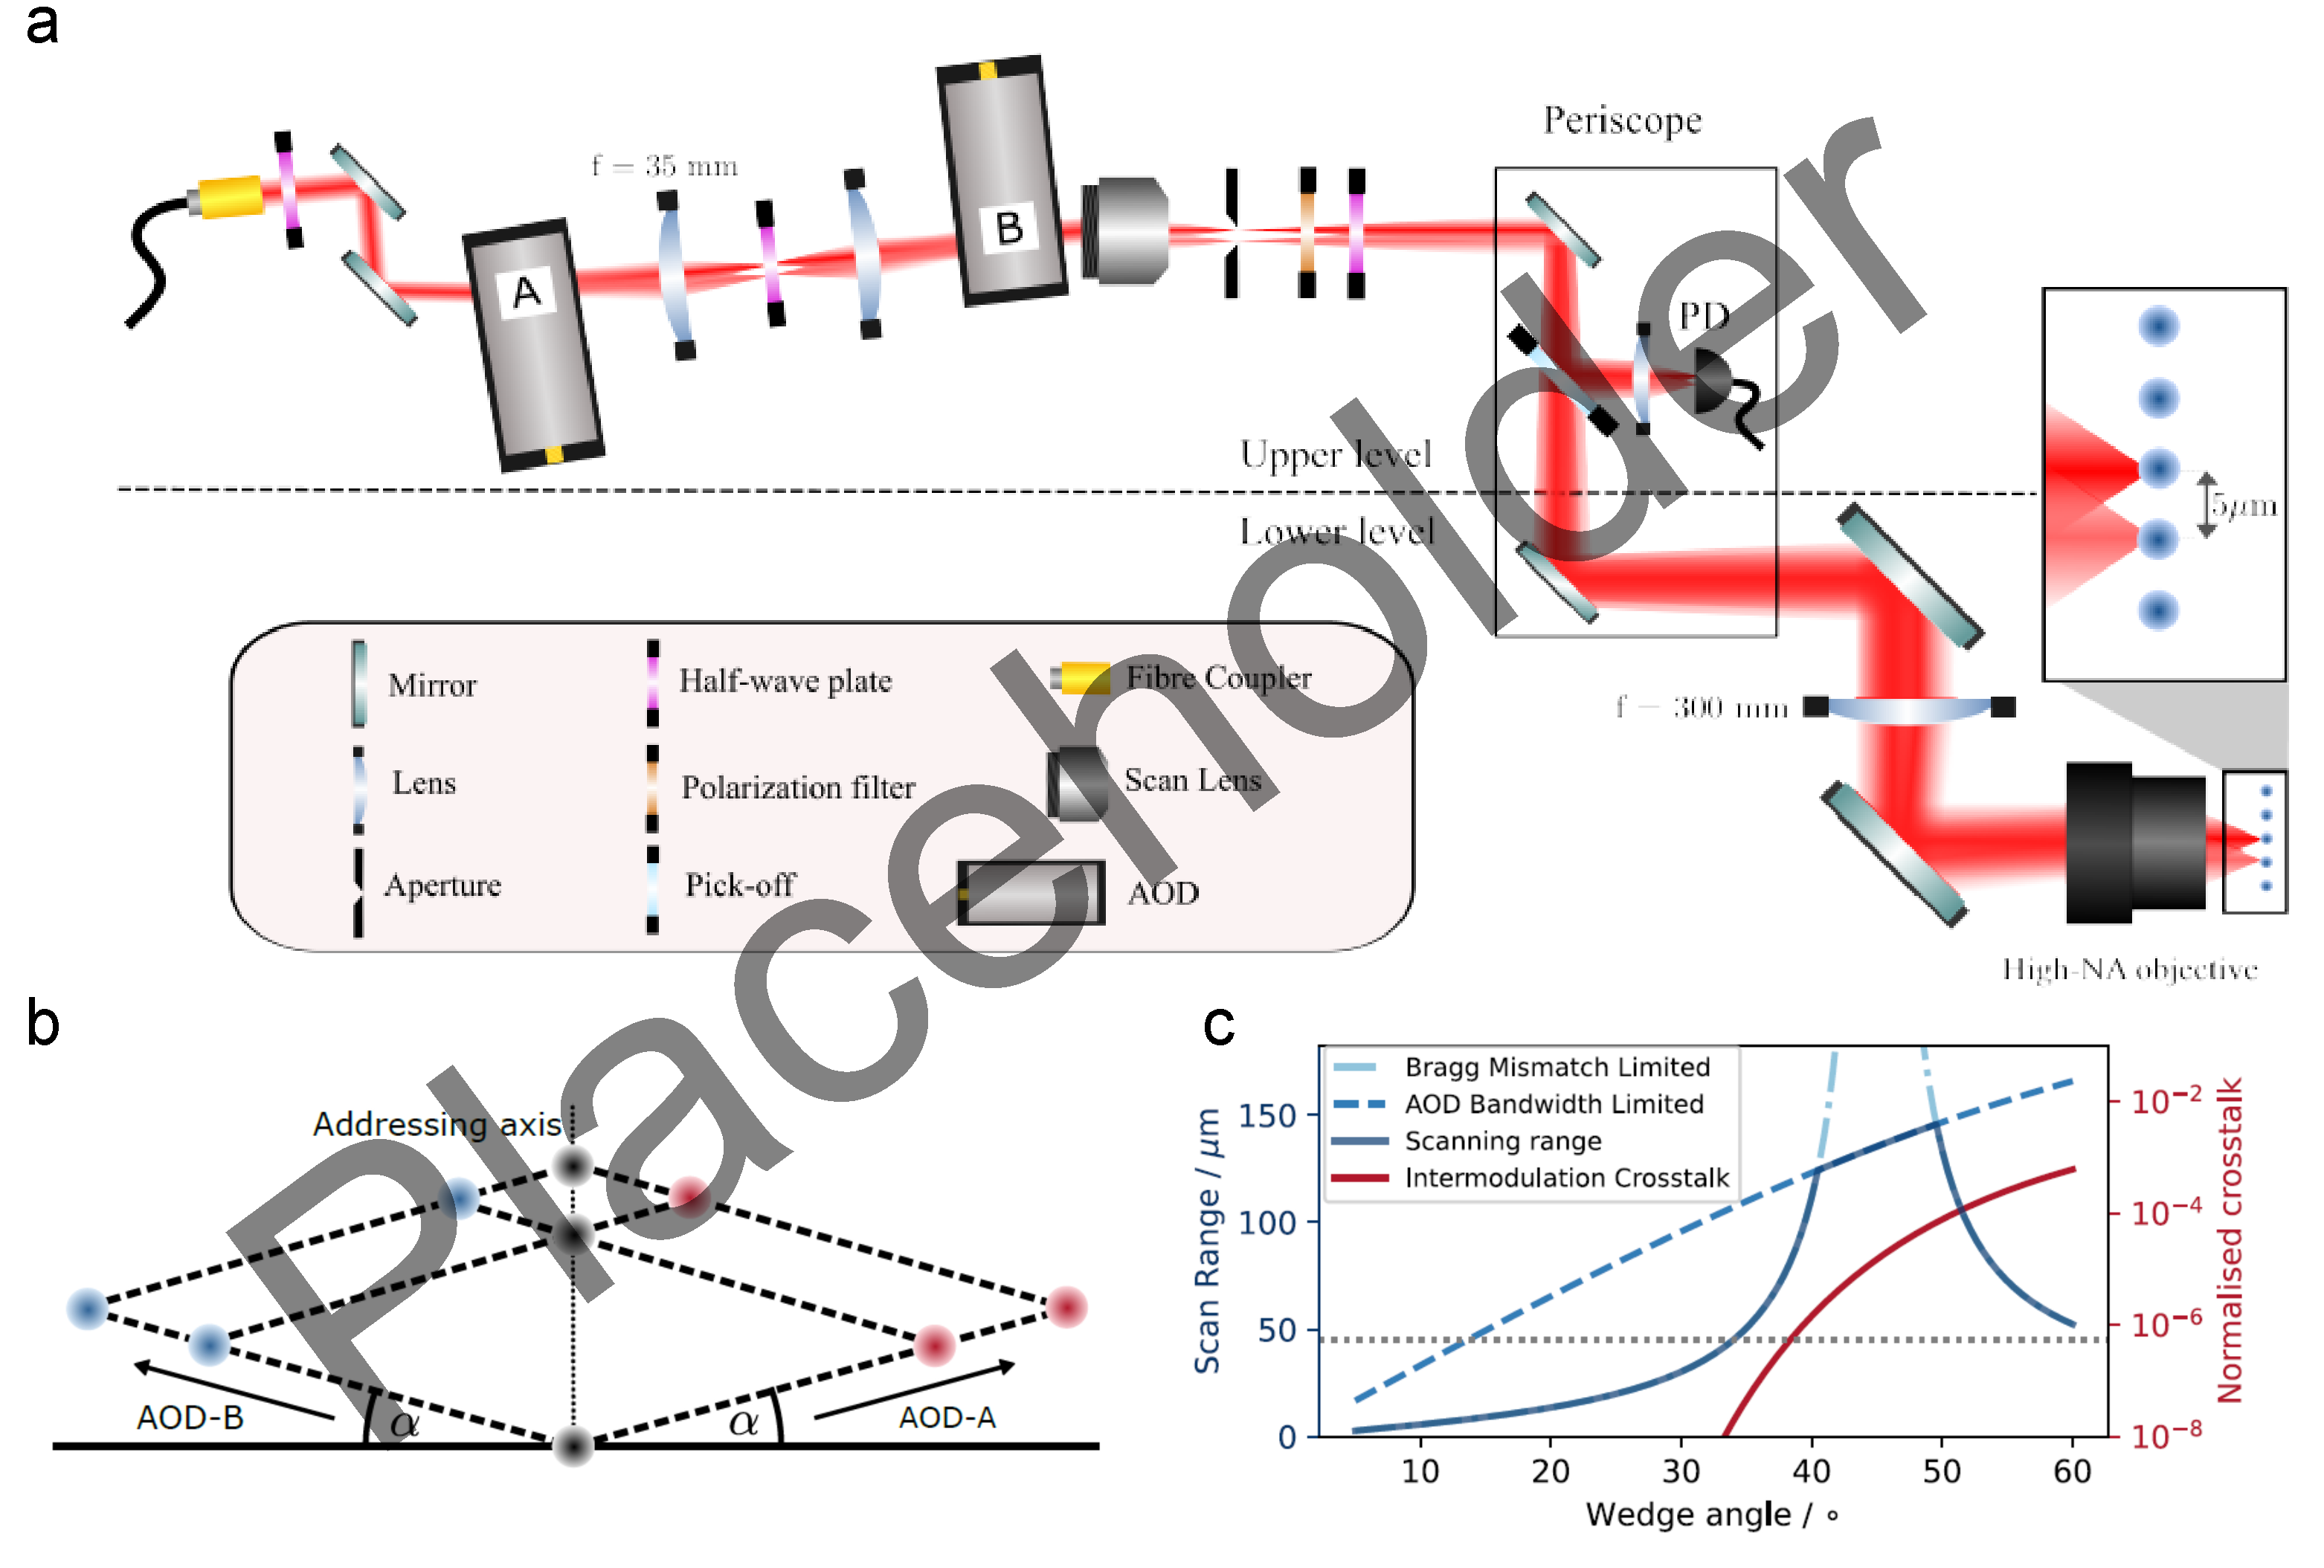
\includegraphics[width=\linewidth]{figures/pdf_figure/ch2/AOD_setup.pdf
        }
    \end{center}
    \caption{
        \todo{Asymptotic population decay for $k>2$ qubits via numerical simulation.}
        }
    \label{fig:AOD}
\end{figure}
% Discuss 1) pairwise generalisation, 2) higher-order correlations, 3) generalising to SLeRB

% ==========================================================================
\section{Analytic predictions for other noise types}
\label{sec:analytic_other_noise}
\todo{Discuss ZZ-type errors, non-unitals, generalised depolarising channels, Stochastic vs coherent errors, etc.}
\begin{figure}
    \begin{center}
    \noindent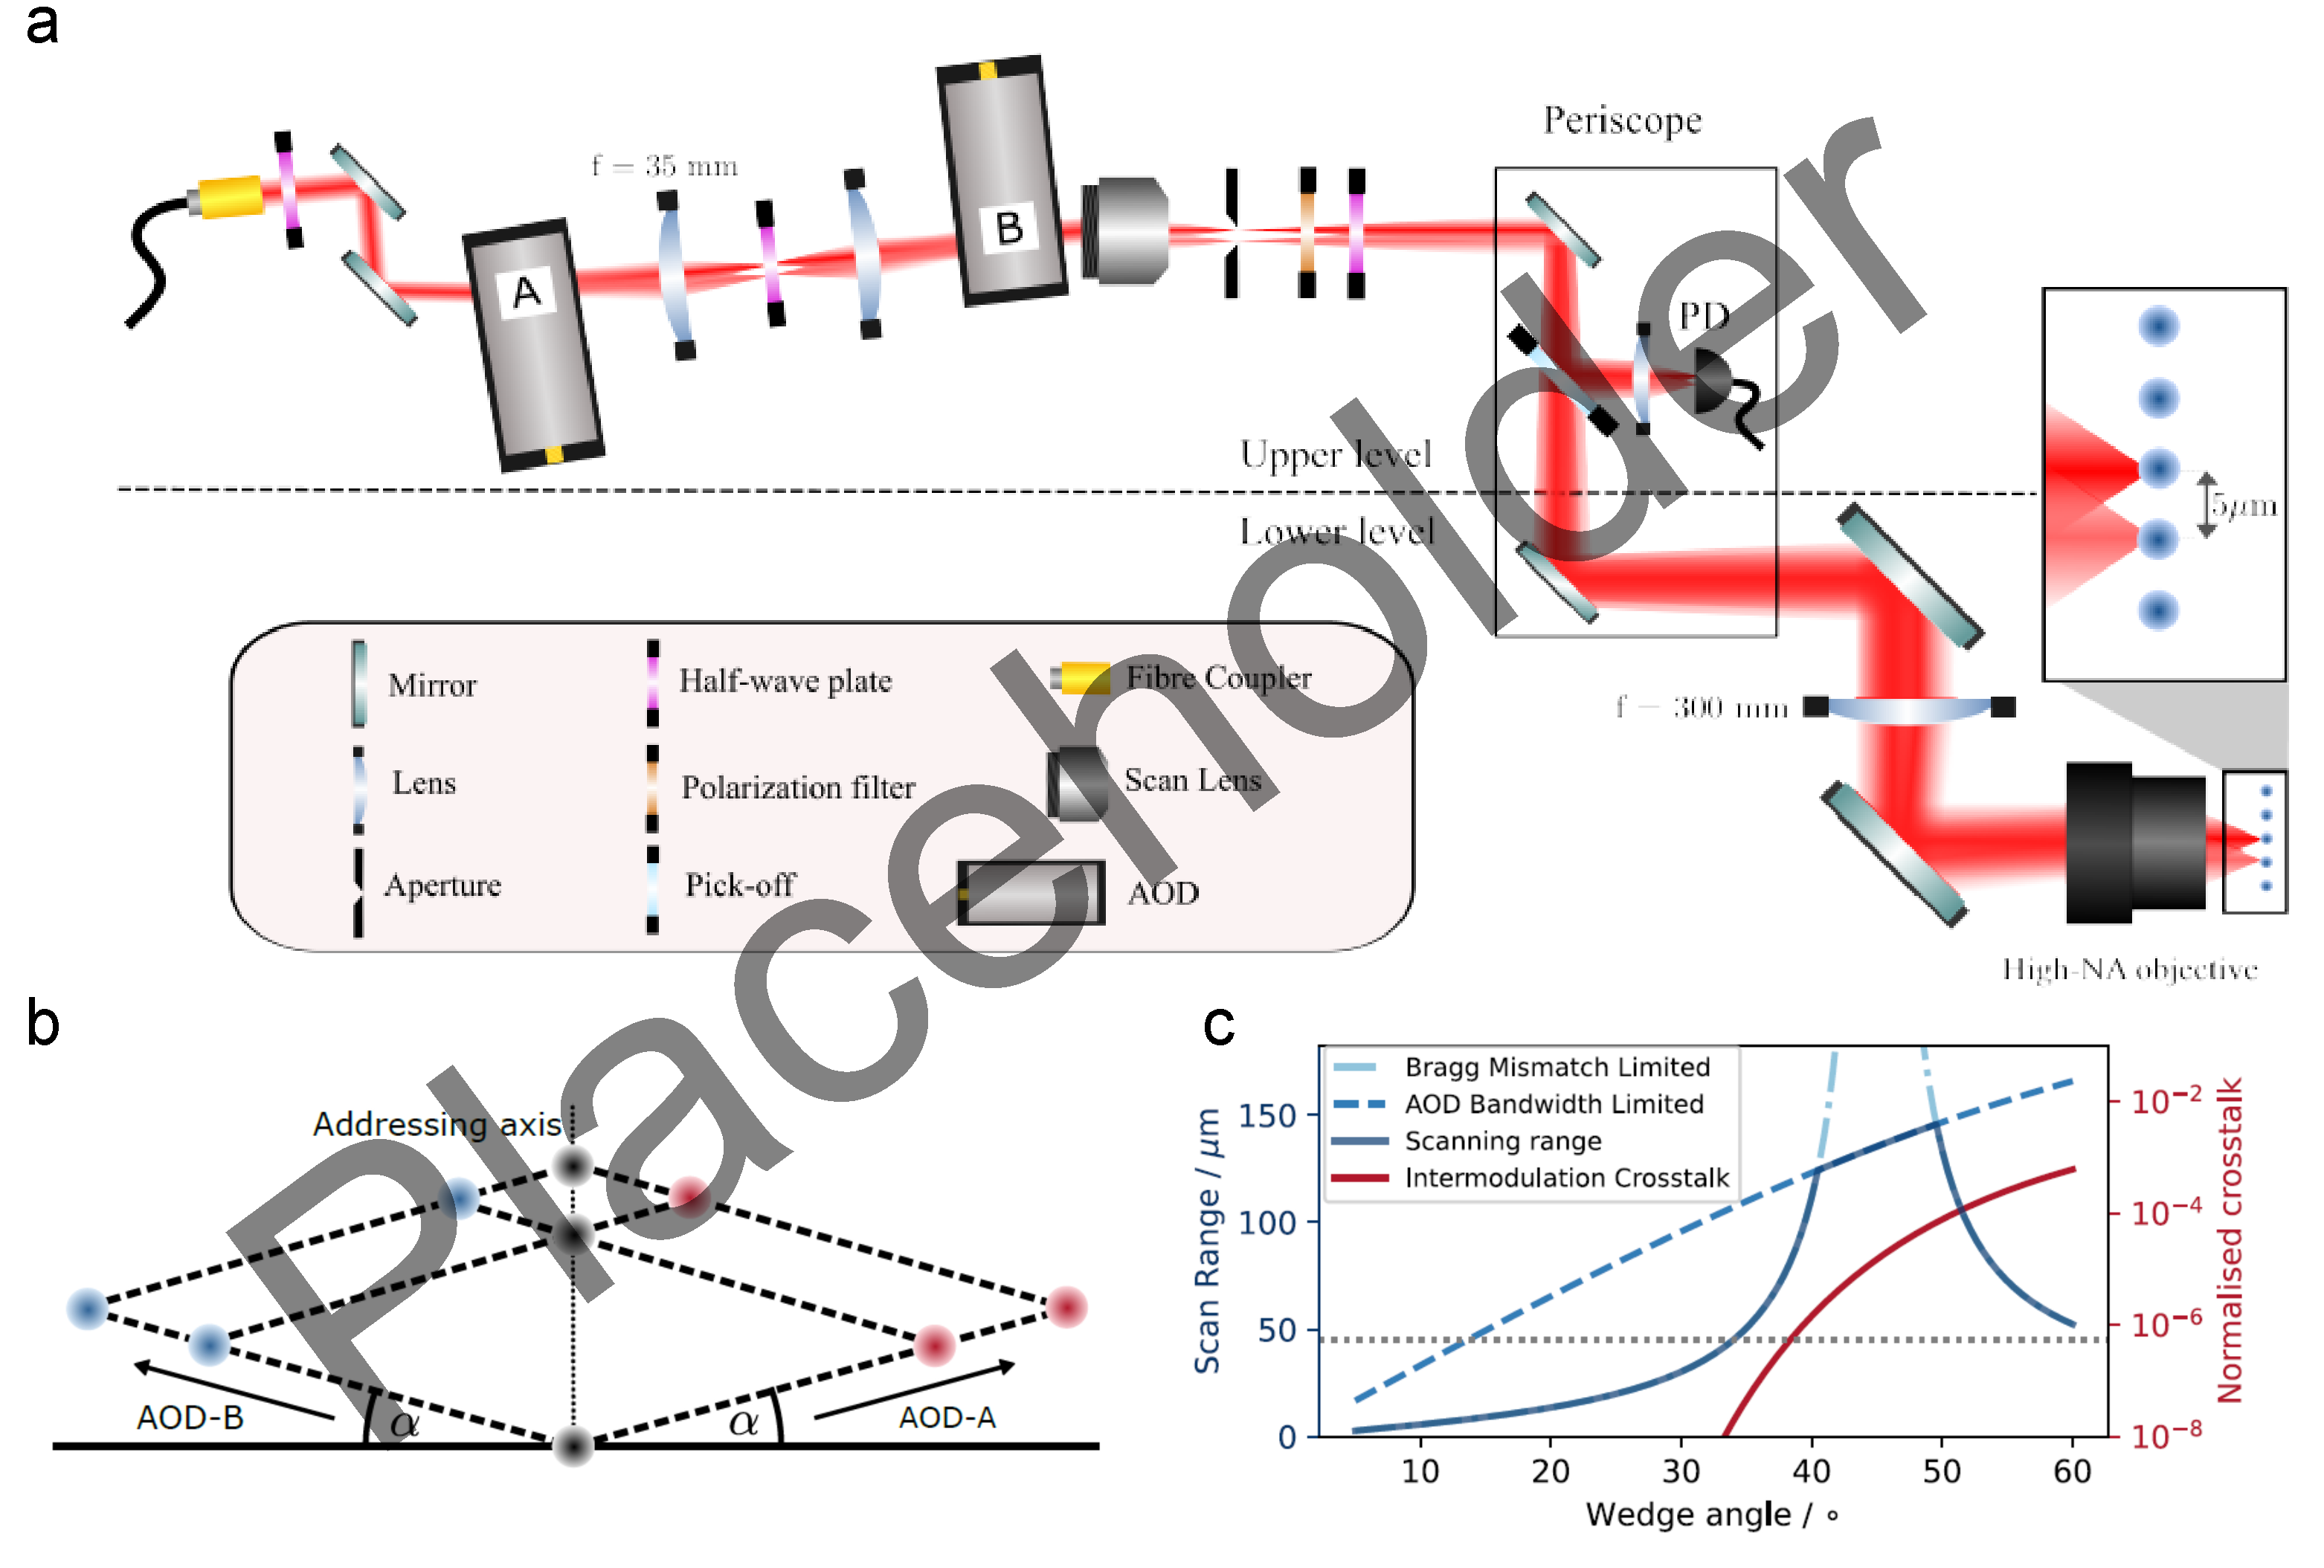
\includegraphics[width=\linewidth]{figures/pdf_figure/ch2/AOD_setup.pdf
        }
    \end{center}
    \caption{
        \todo{Liouville-block structure for other noise types.}
        }
    \label{fig:AOD}
\end{figure}

\section{Results}
\label{sec:results}

\subsection{Discerning correlated and uncorrelated error}
\label{sec:results_discern}

The 24 single-qubit Clifford gates
are decomposed into native single-qubit rotations of the form
$\hat R_x(\pi/2)$ and $\hat R_z(\pi/2)$: $\hat\sigma_x$ rotations are
performed natively on resonance with the qubit transition, with relative
phase set by modulating the \SI{729}{\nano\meter} beam via an
acousto-optic modulator (AOM), while $\hat\sigma_z$ rotations are performed
virtually by updating the phase of subsequent $\hat\sigma_x$ rotations.

\subsubsection{$Z$-basis measurements}

\begin{figure}
    \begin{center}
    \noindent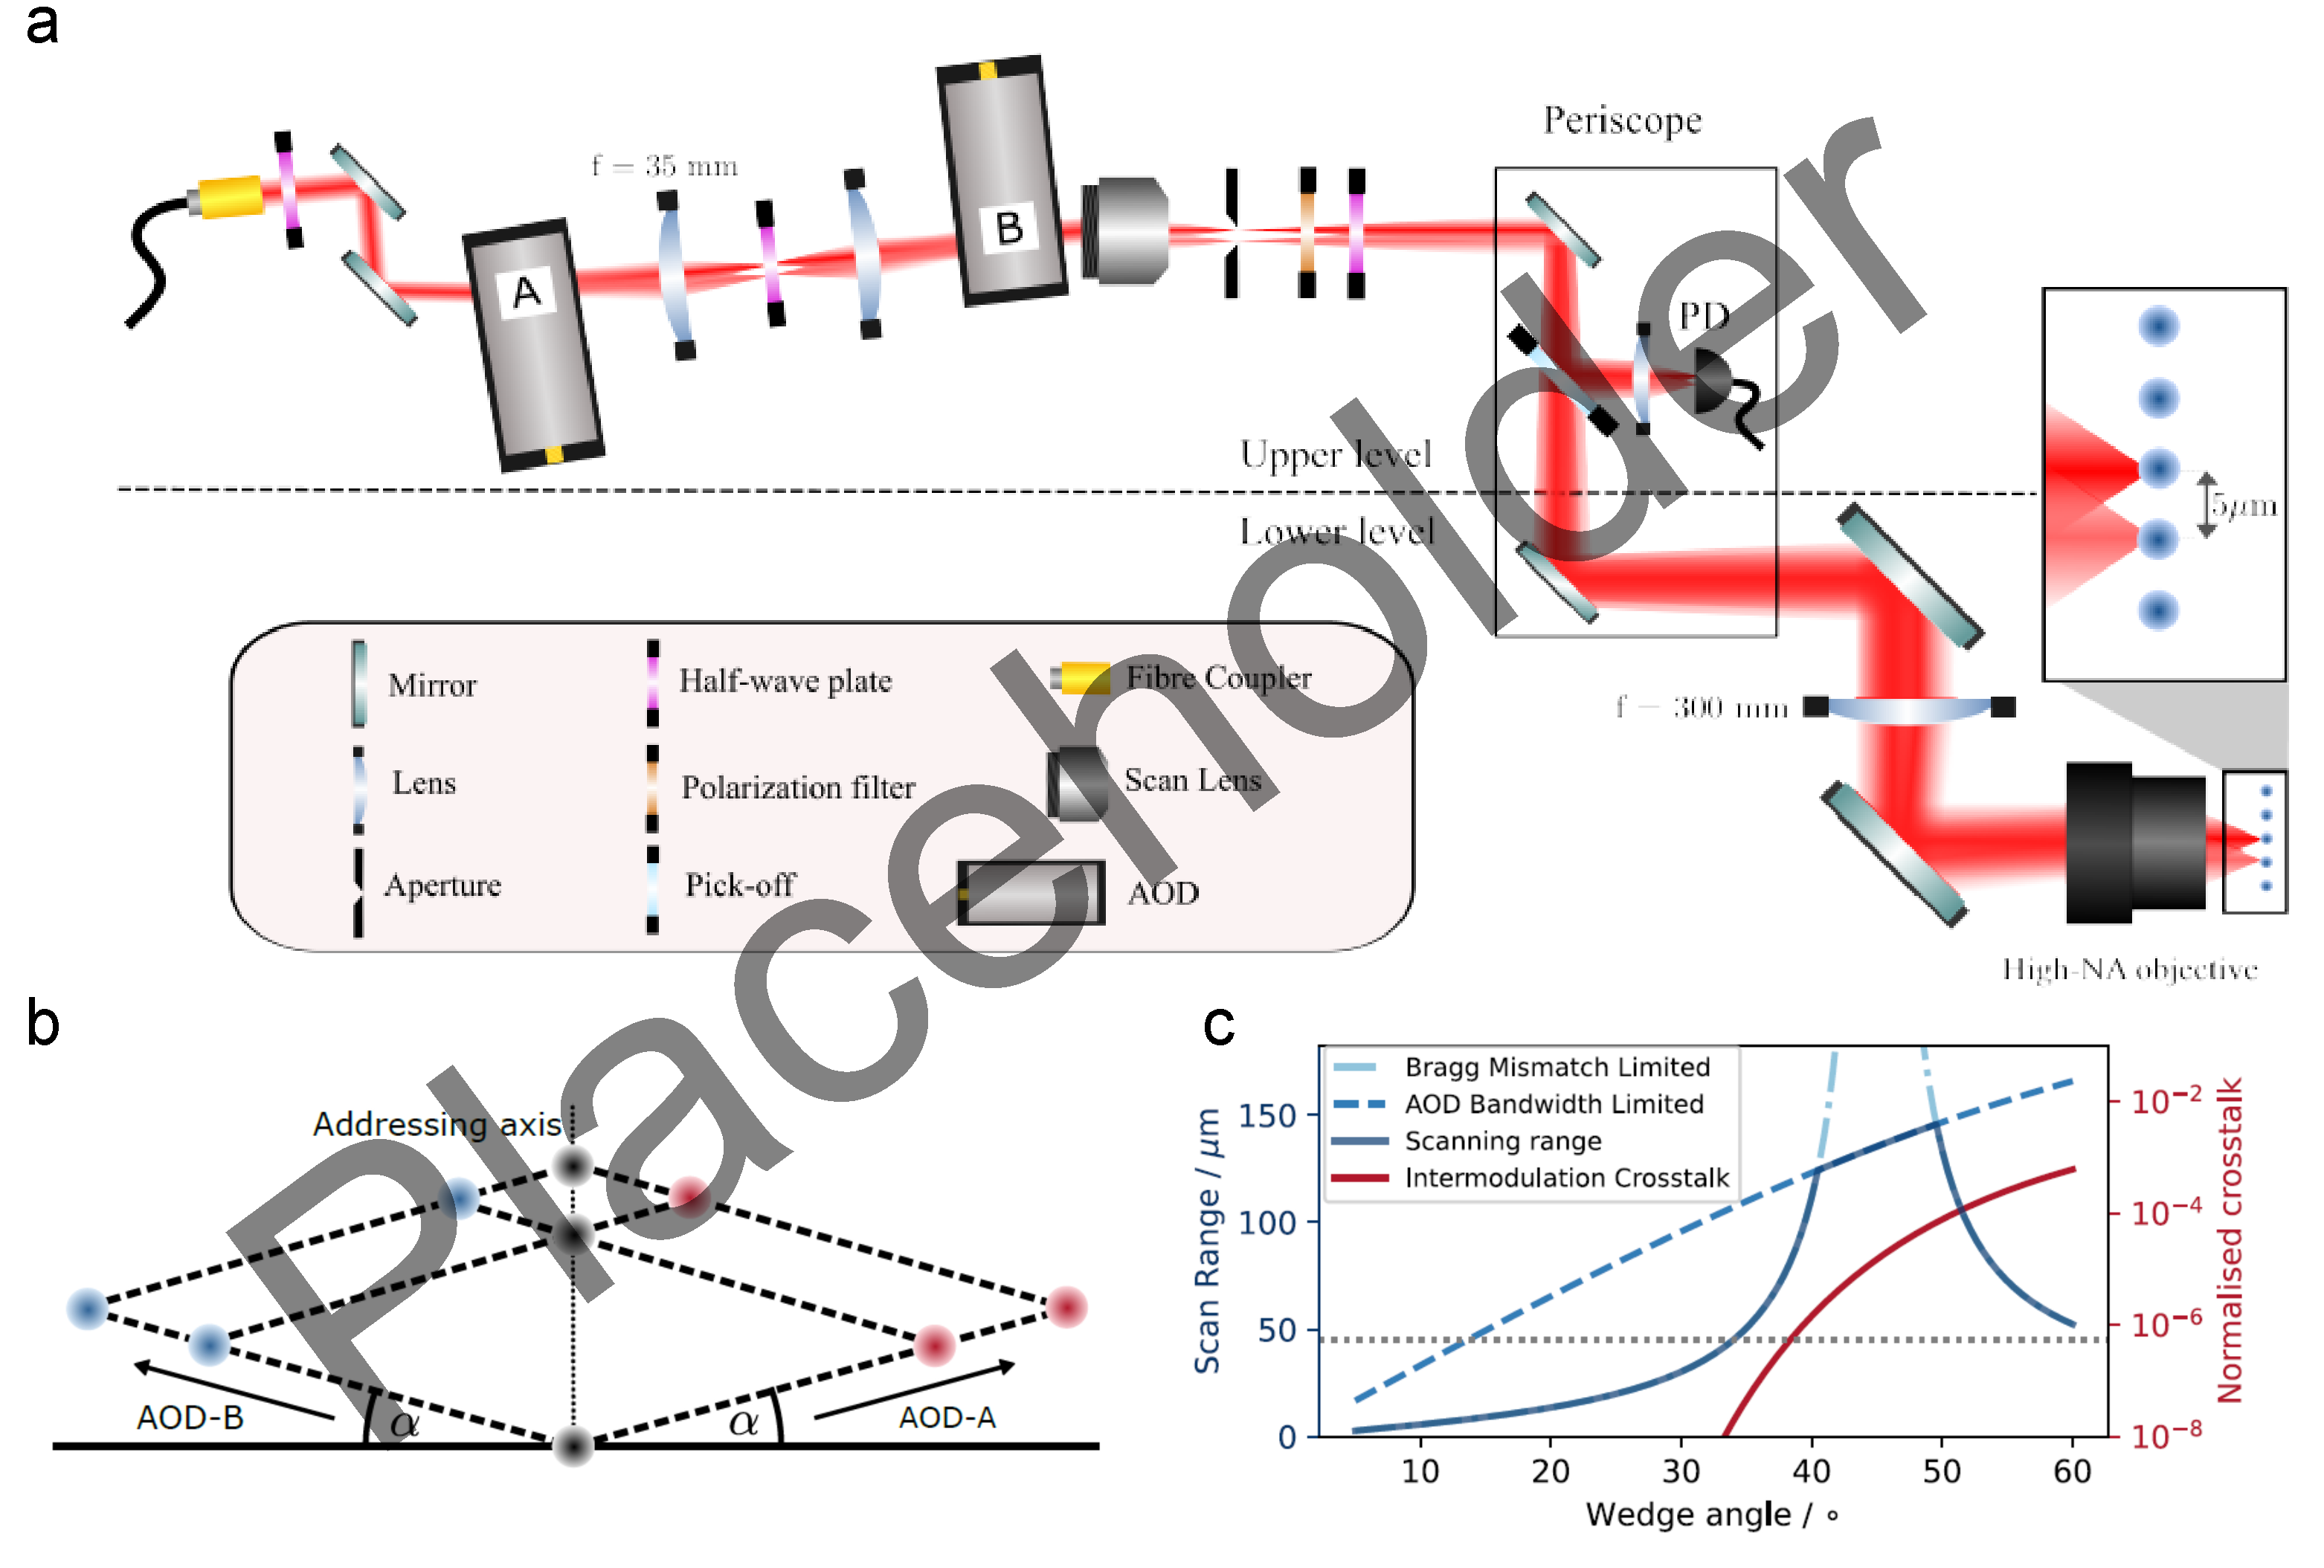
\includegraphics[width=\linewidth]{figures/pdf_figure/ch2/AOD_setup.pdf
        }
    \end{center}
    \caption{
        \todo{Exp data from fig 2 a,b,c}
        }
    \label{fig:AOD}
\end{figure}
$k$-copy RB is first demonstrated in a regime where common noise is the
dominant error source, induced via a fixed \SI{10}{\kilo\hertz} frequency
detuning of the \SI{729}{\nano\meter} laser. Standard single-qubit RB decay
curves (Section~\ref{sec:standard_rb}) are recorded alongside two-qubit
correlated populations extracted via $k$-copy RB.

\todo{(a,b) single-qubit RB decays; (c) two-qubit correlated
success population $P_{SS}$ vs.\ sequence length; (d) parity contrast vs.\
sequence length, with example fringe insets.}{Correlated two-qubit
probabilities discern correlated and uncorrelated error channels (adapted
from manuscript Fig.~2). \todo{Redraw for thesis; consider separating
panels (a,b) [standard RB, Section~\ref{sec:standard_rb} recap] from (c,d)
[the $k$-copy-specific result] into two figures for pedagogical clarity.}}

The correlated populations exhibit a clear intermediate asymptote at
$m \approx 100$ Cliffords, corresponding to the initial state $\ket{00}$
approaching $\rho_{sym}$ (Eq.~\eqref{eqn:bell}), followed by a slower decay
to the fully depolarised two-qubit state by $m \approx 1000$. These two
decay rates, corresponding to correlated and uncorrelated error
respectively, are indistinguishable in the single-qubit decays and are only
revealed through the correlated measurements made during $k$-copy RB.
Fitting Eq.~\eqref{eqn:decay} gives extracted parameters
$\varepsilon_\mathrm{corr}=0.051(3)$, $\varepsilon_L=0.001(1)$, and
$\varepsilon_R=0.000(1)$.

\subsubsection{Coherence measurements}
\begin{figure}
    \begin{center}
    \noindent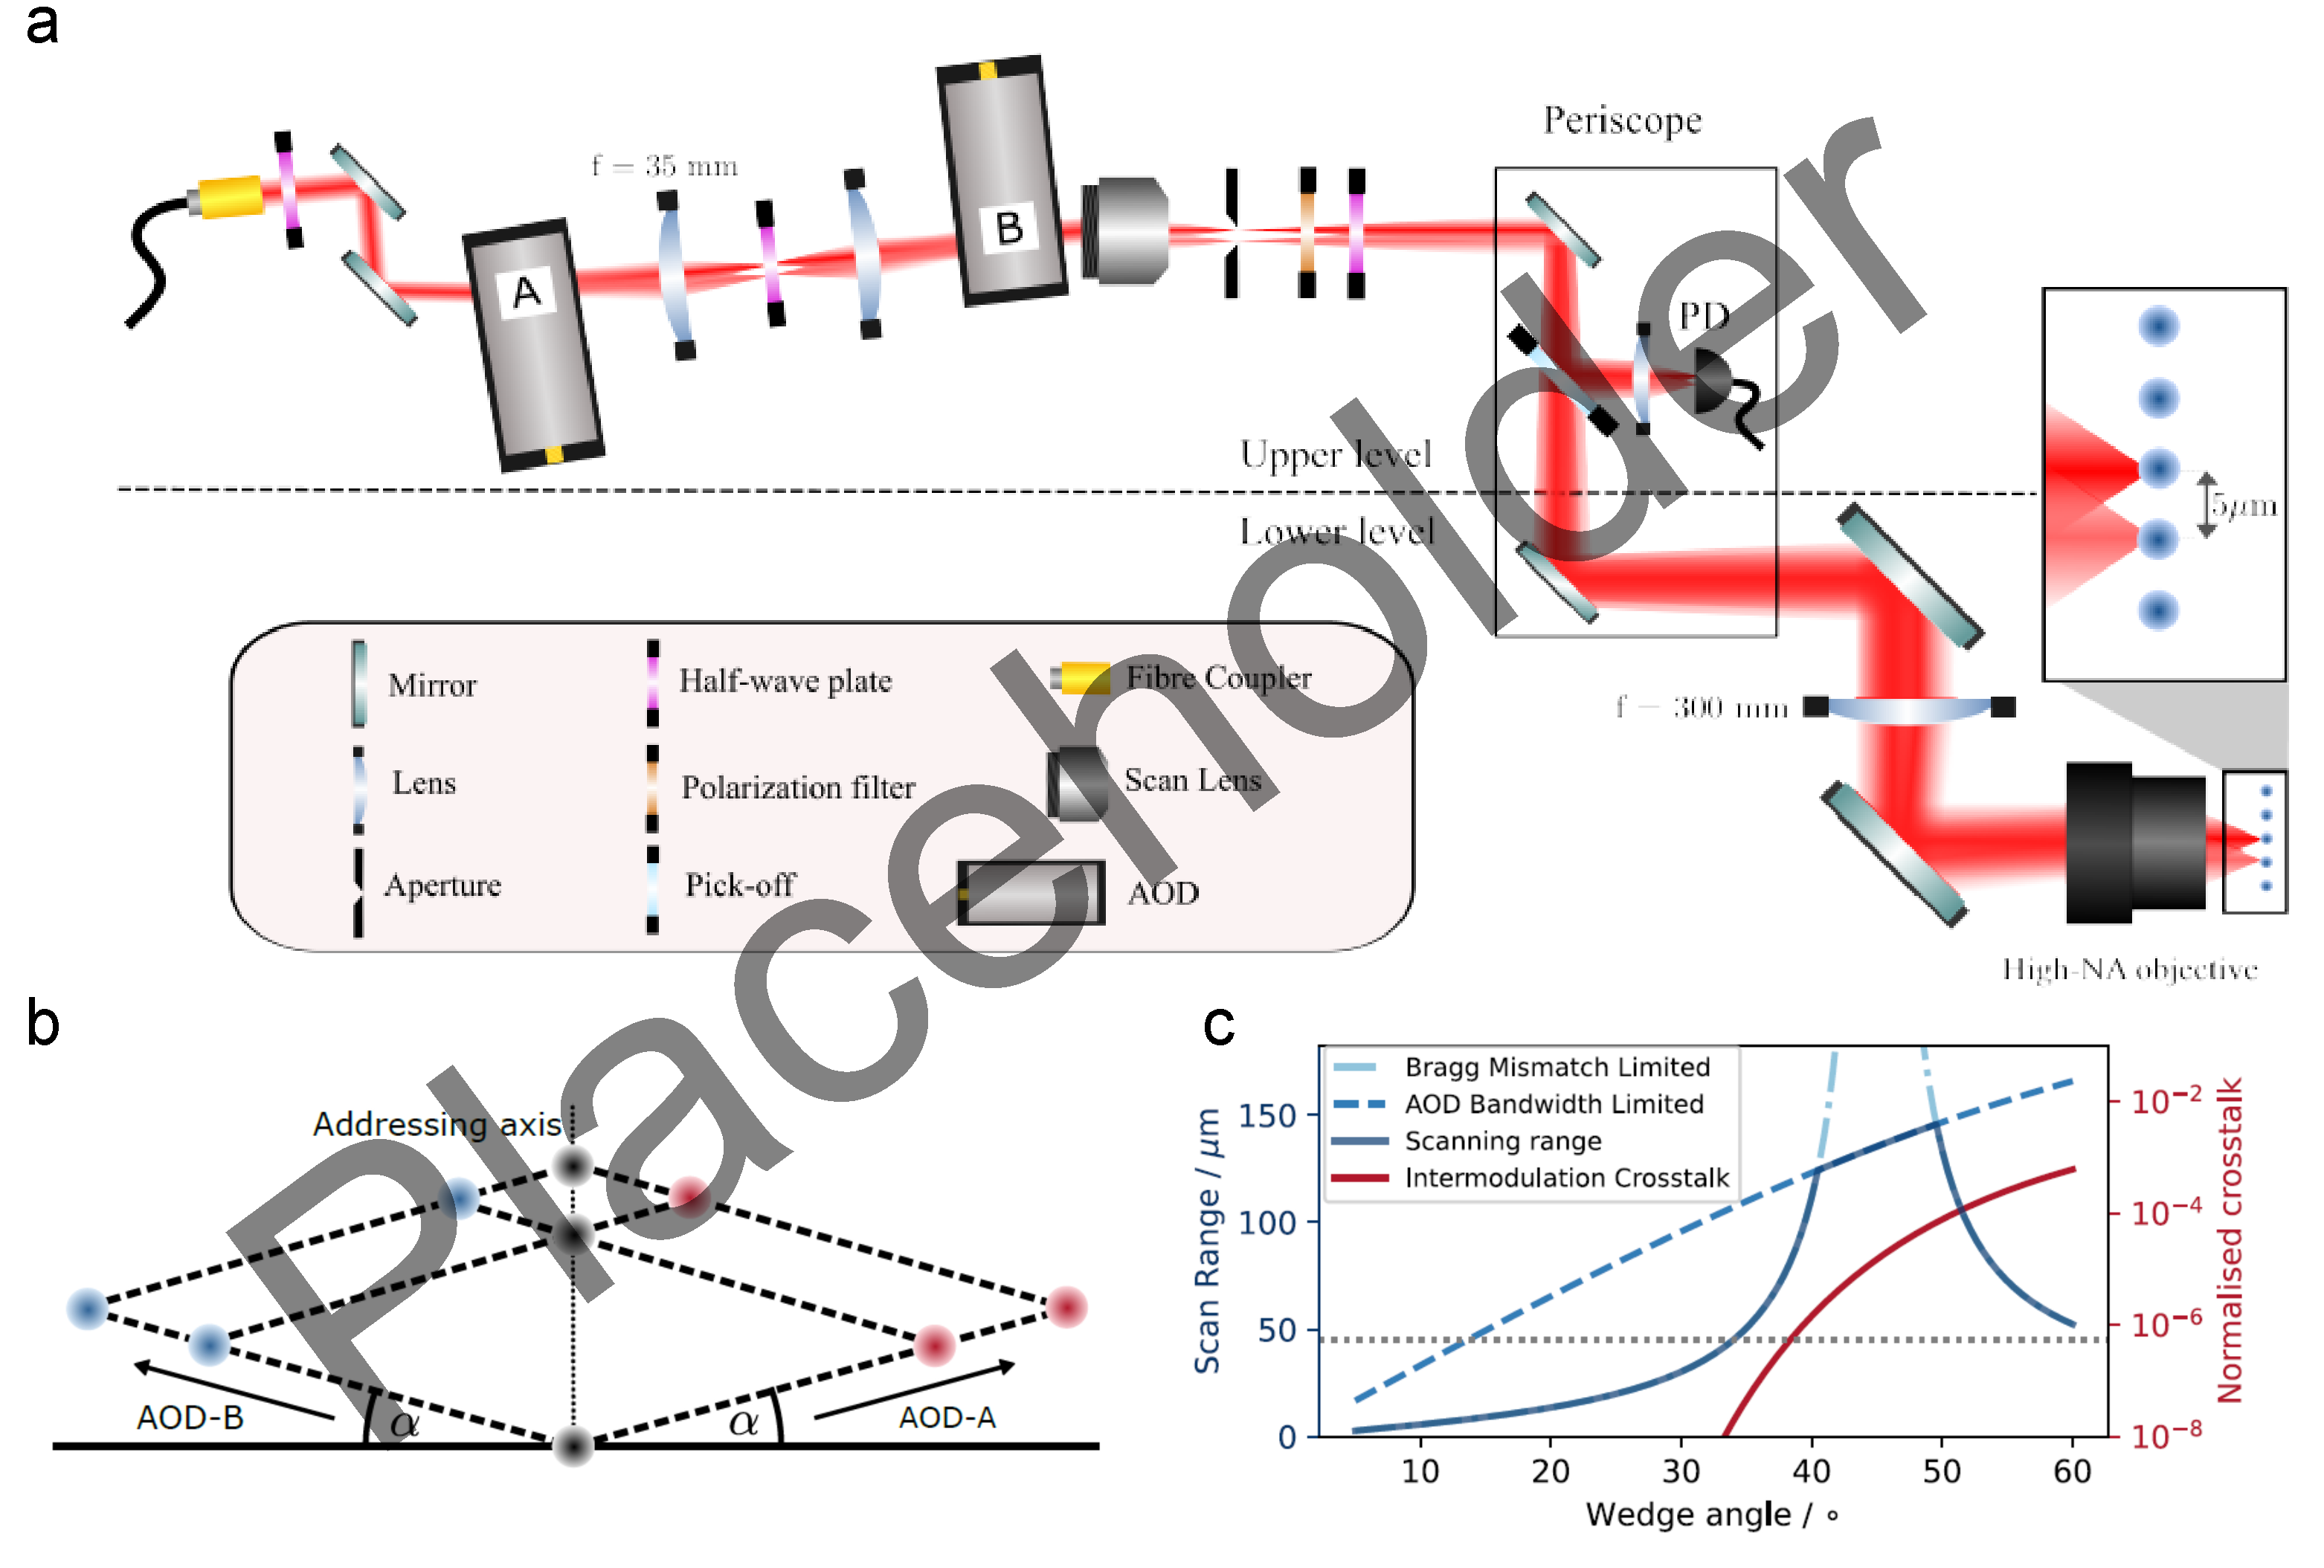
\includegraphics[width=\linewidth]{figures/pdf_figure/ch2/AOD_setup.pdf
        }
    \end{center}
    \caption{
        \todo{Exp data from fig 2 d + parity oscillations.}
        }
    \label{fig:AOD}
\end{figure}
A partial-tomography parity measurement (Section~\ref{sec:parity}) is used
to independently confirm occupation of the symmetric sector, quantifying
overlap of the final state with $\ket{\Psi^+}$. The expected contrast
asymptote $\mathcal{C}\to 1/3$ (Eq.~\eqref{eqn:parity}) is observed for
$m \in [10,100]$, corresponding to residual two-qubit coherence. Fitting
Eq.~\eqref{eqn:parity} gives $\varepsilon_\mathrm{corr}=0.043(3)$ and
$\varepsilon_L=\varepsilon_R=0.0016(1)$; the increased depolarising rate
relative to the population fit is attributed to imperfect execution of the
$R_{\pm\phi}(\pi/2)$ pulses used for the addressed differential rotation.

\todo{Add explicit discussion/reconciliation of the discrepancy between the
$\varepsilon_L, \varepsilon_R$ values extracted from the population fit vs.\
the parity fit --- the manuscript attributes this briefly to addressing-beam
imperfections but a thesis chapter could quantify this more carefully (e.g.\
independently characterising the single-addressing system's contribution).}

\subsection{Controlled noise injection}
\subsubsection{Numerical simulations of correlated vs.\ uncorrelated noise}
% Here could have the numerics for sample cost
\begin{figure}
    \begin{center}
    \noindent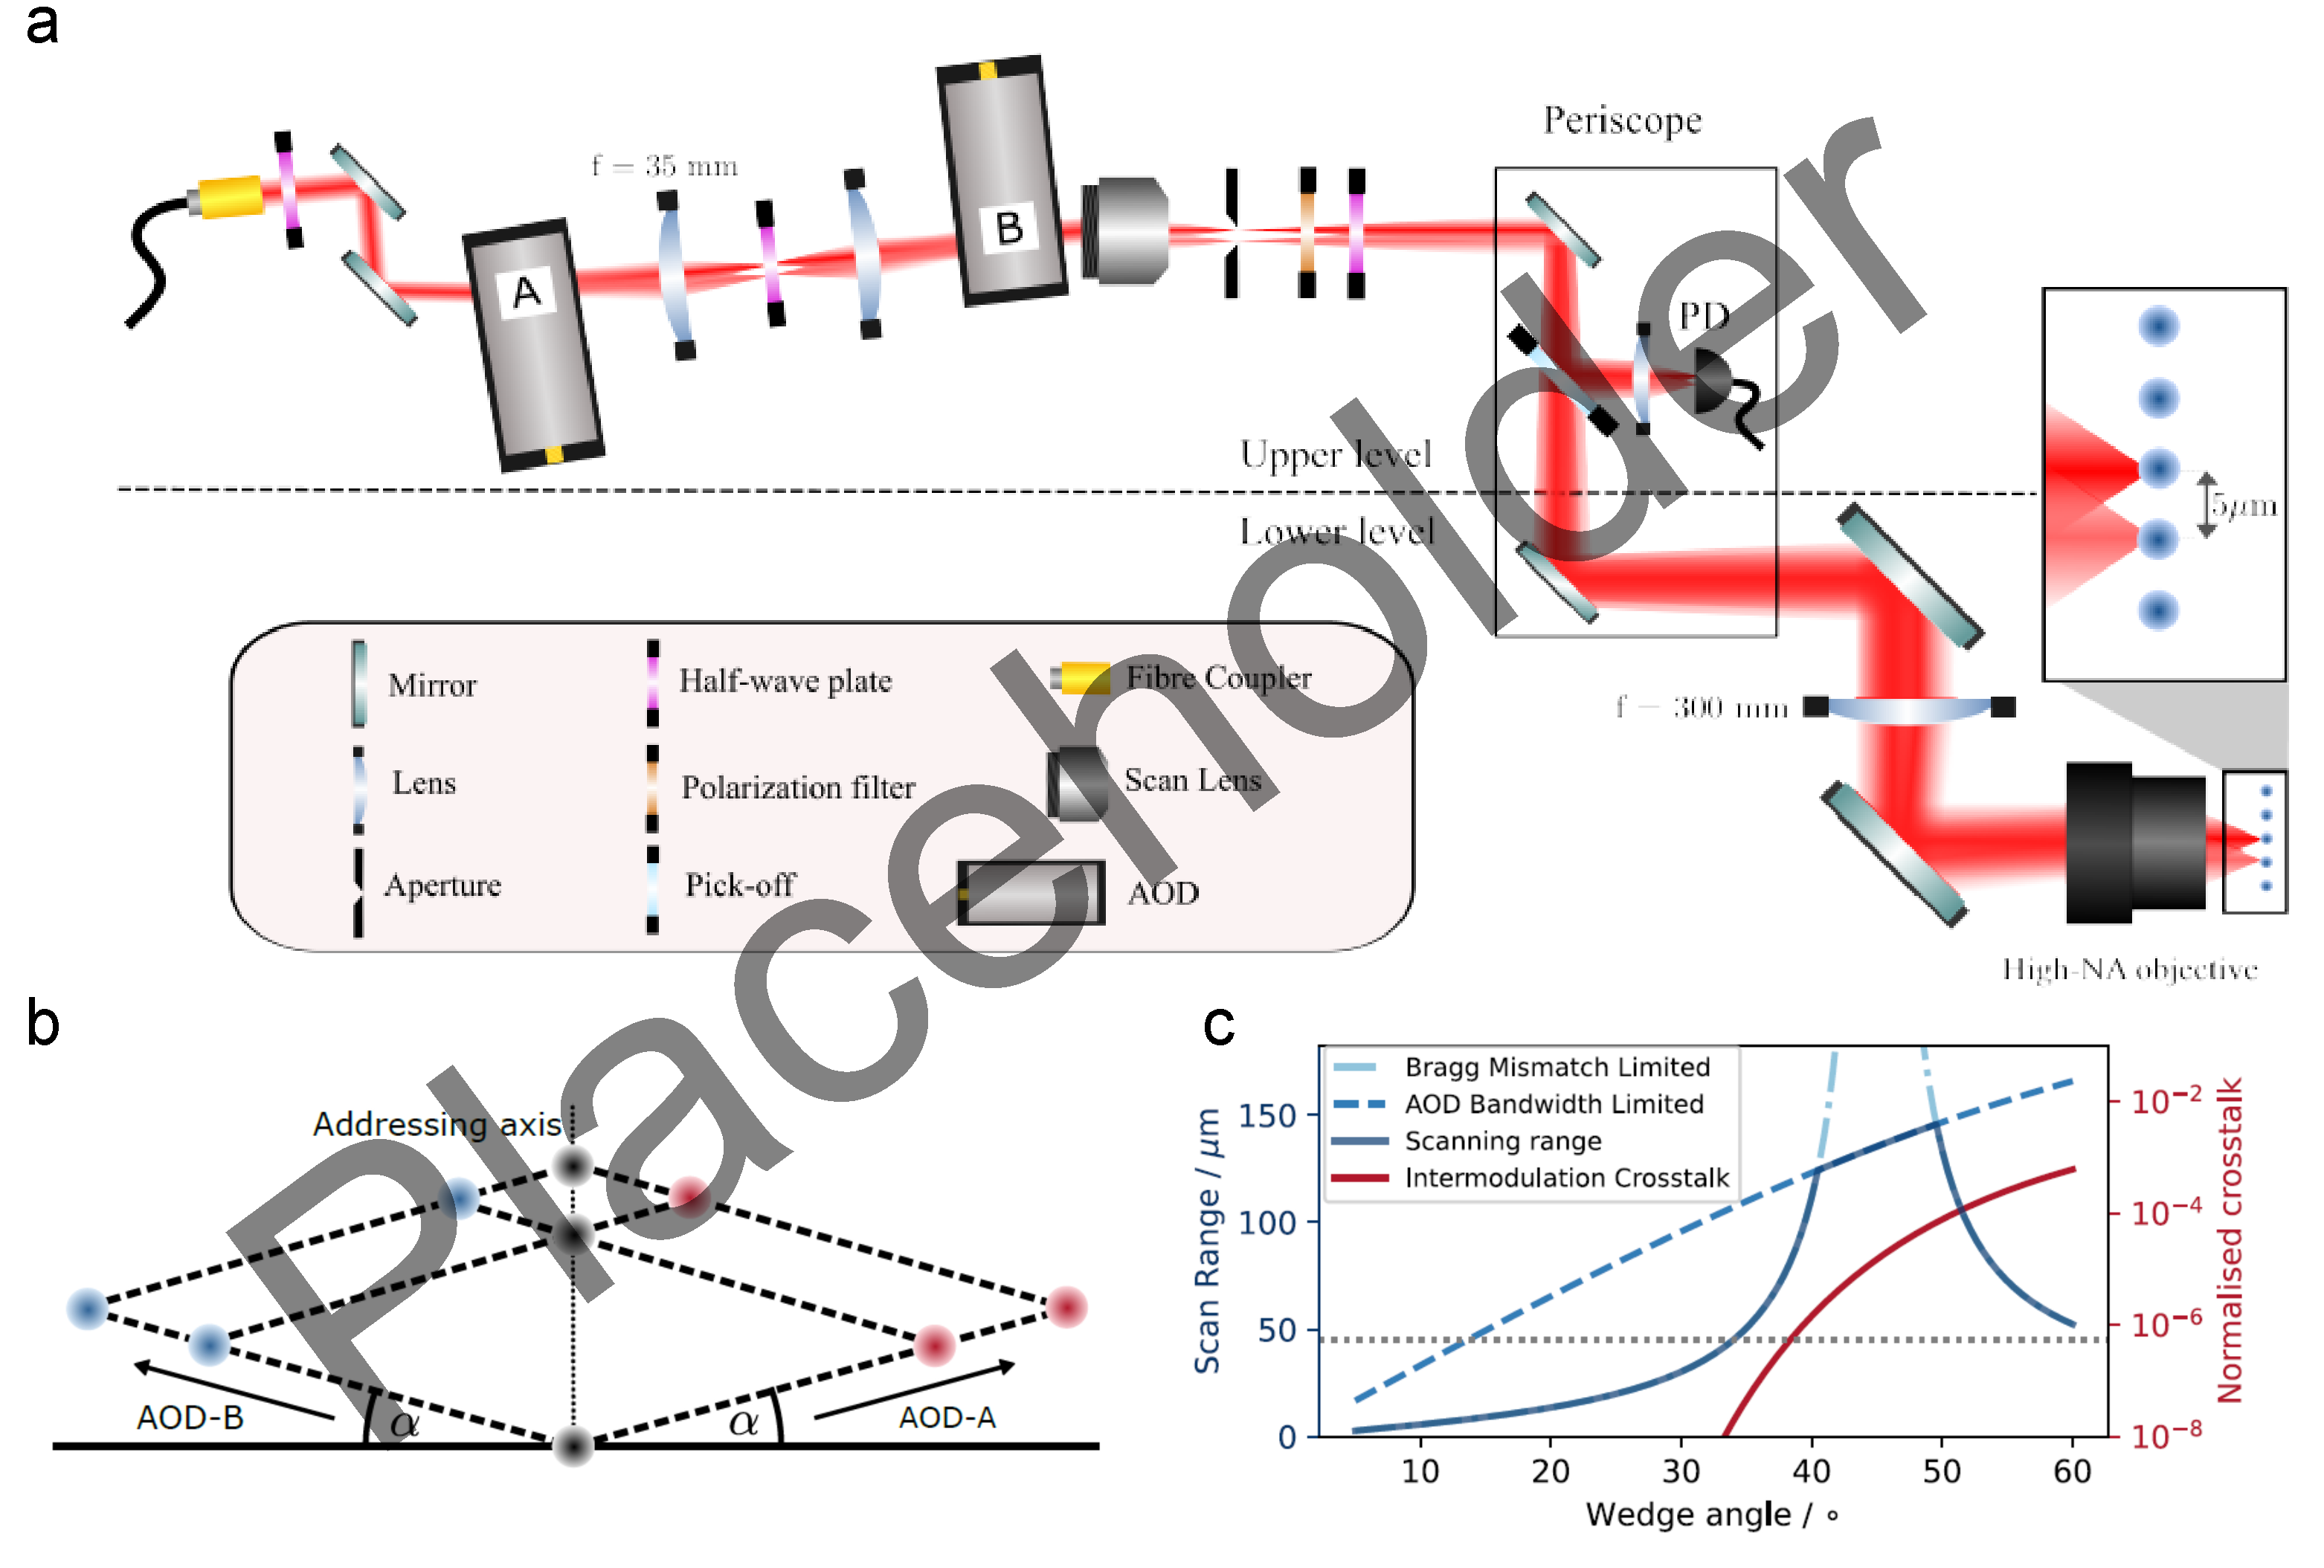
\includegraphics[width=\linewidth]{figures/pdf_figure/ch2/AOD_setup.pdf
        }
    \end{center}
    \caption{
        \todo{Numerical sim of param space and extracted fit uncertainties.}
        }
    \label{fig:AOD}
\end{figure}

\subsubsection{laser phase jitter}
\label{sec:phase_jitter}
\begin{figure}
    \begin{center}
    \noindent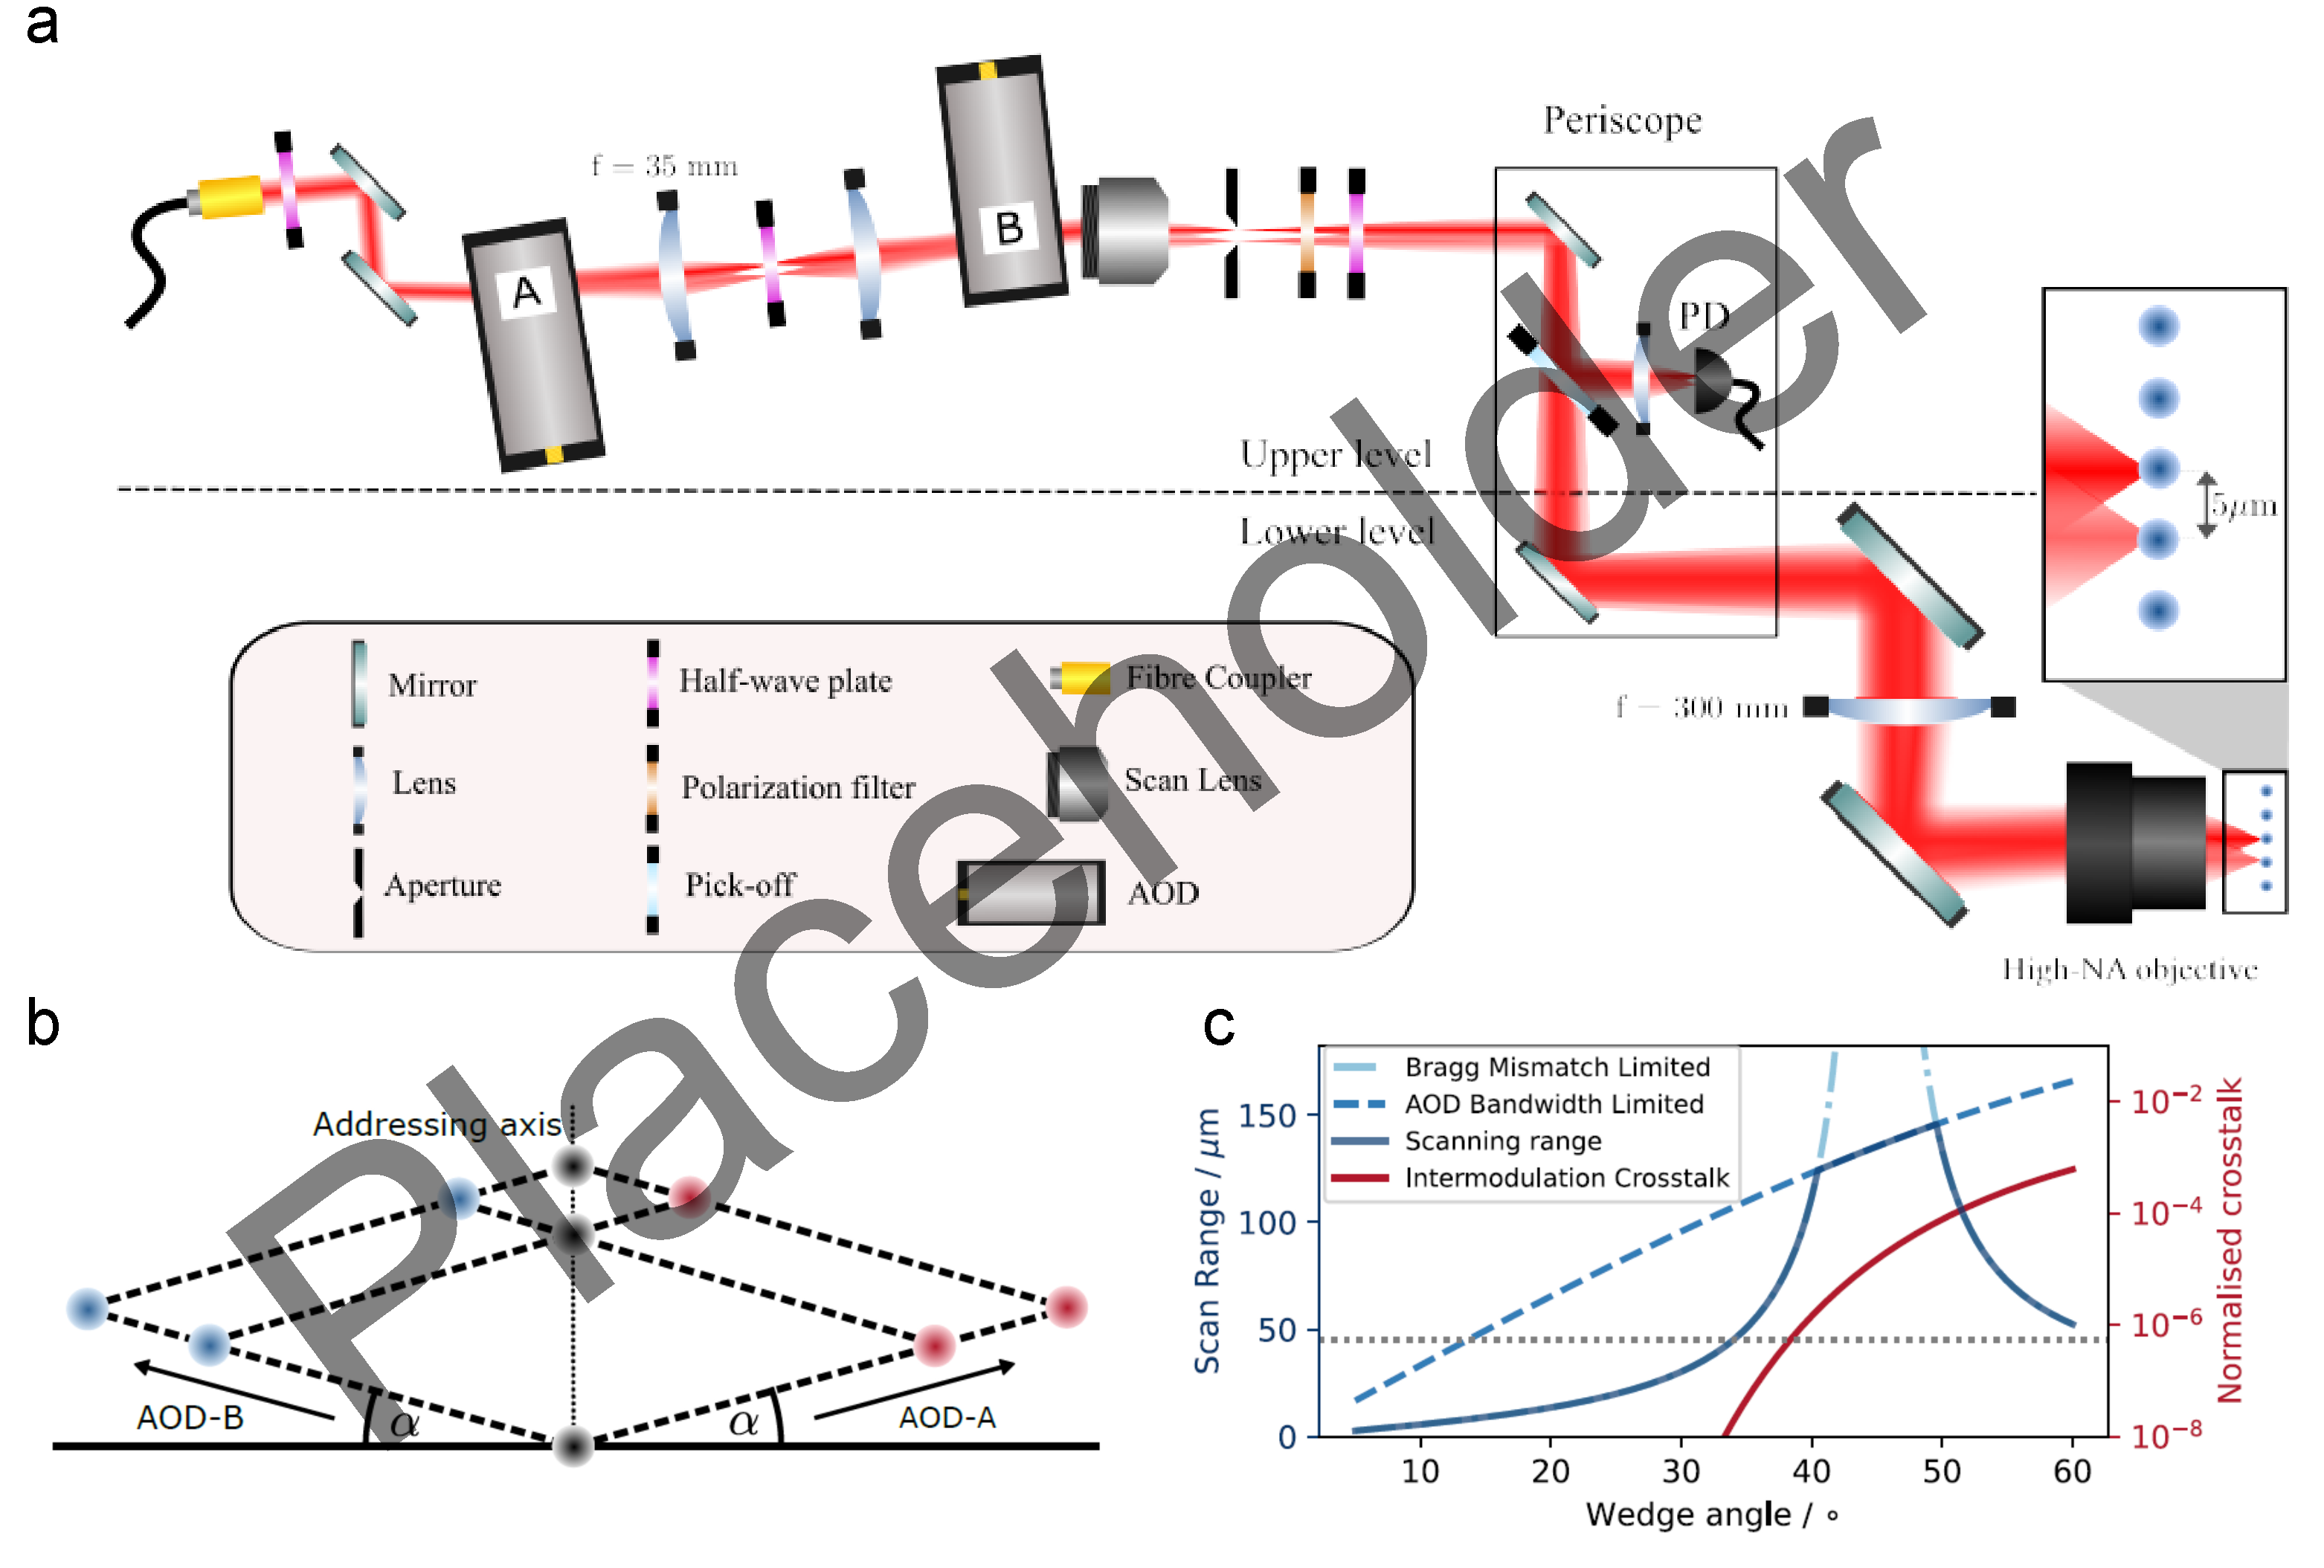
\includegraphics[width=\linewidth]{figures/pdf_figure/ch2/AOD_setup.pdf
        }
    \end{center}
    \caption{
        \todo{Injecting phase jitter calibration}
        }
    \label{fig:AOD}
\end{figure}

\subsubsection{laser detuning scan}
\label{sec:detuning_scan}

\begin{figure}
    \begin{center}
    \noindent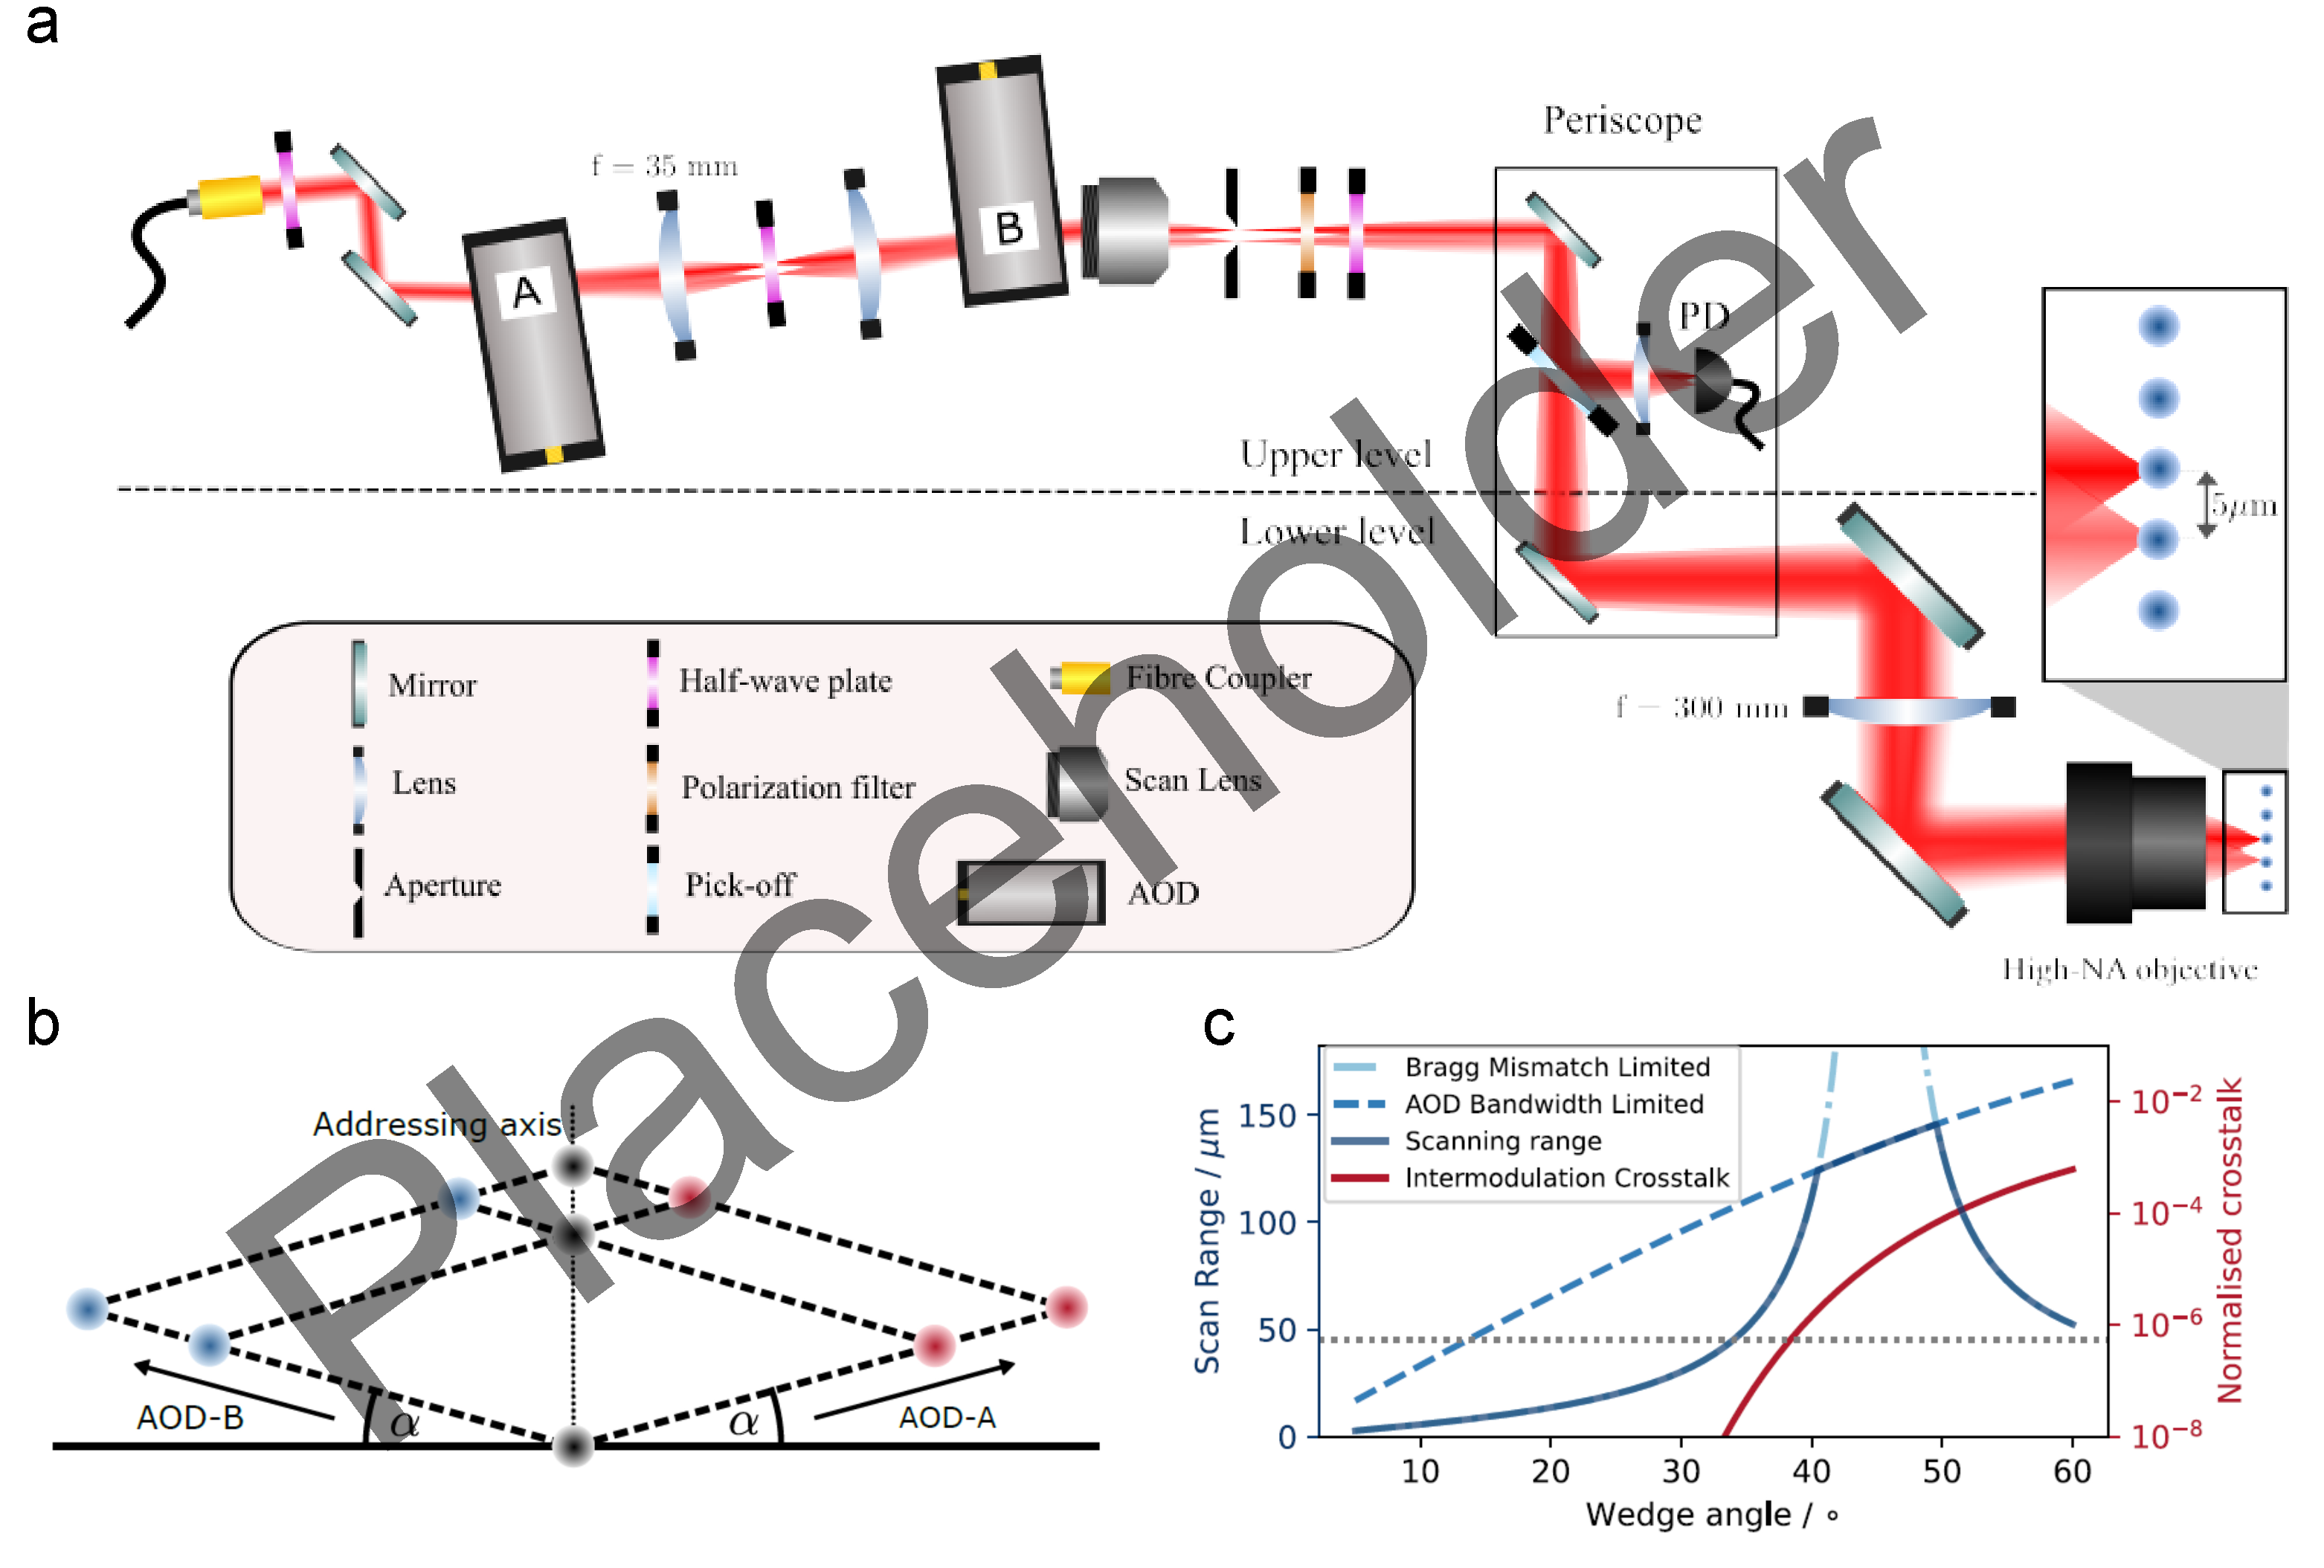
\includegraphics[width=\linewidth]{figures/pdf_figure/ch2/AOD_setup.pdf
        }
    \end{center}
    \caption{
        \todo{figure 3 from paper.}
        }
    \label{fig:AOD}
\end{figure}
$k$-copy RB can isolate errors arising from shared control fields, making it
useful both for device characterisation and for optimising global control
parameters. This is demonstrated by scanning the \SI{729}{\nano\meter}
laser frequency used for single-qubit rotations away from the bare qubit
resonance.

\todo{Upper: example correlated populations for several detuning
values. Lower: extracted correlated ($\varepsilon_{\mathrm{corr}}$, red) and
local ($\varepsilon_L,\varepsilon_R$, blue) error per Clifford vs.\
detuning, with quadratic fit.}{Correlated errors injected via detuning of a
shared drive laser (adapted from manuscript Fig.~3). \todo{Redraw for
thesis.}}

Each data point is obtained from a complete $k$-copy RB experiment with 11
sequence lengths up to $m=1024$, using $r=50$ random sequences and $s=50$
shots per sequence, with correlated populations fit to Eq.~\eqref{eqn:decay}
to extract $\{\varepsilon_{\mathrm{corr}}, \varepsilon_L, \varepsilon_R\}$
at each detuning. The correlated error is observed to increase
quadratically with detuning, while the local depolarising errors remain
approximately constant, consistent with detuning of a shared drive
producing common noise as defined in Section~\ref{sec:common_noise}. This
dependence is modelled as
\begin{equation}
    \varepsilon_{corr} = \varepsilon_0 + \frac{\kappa}{3}
    \left(\frac{\delta_L - \delta_0}{\Omega}\right)^2,
    \label{eqn:detuning_model}
\end{equation}
where $\varepsilon_0$ is the residual correlated error not originating from
detuning, $\delta_0$ accounts for the light-shifted resonance,
$\Omega = 2\pi\times\SI{100(1)}{\kilo\hertz}$ is the independently measured
Rabi frequency, and $\kappa$ depends on the Clifford decomposition to
hardware-native gates. Fitting gives $\varepsilon_0 = 3.2(1)\times10^{-3}$,
$\kappa = 15.9(7)$, and $\delta_0 = 2\pi \times \SI{0.80(5)}{\kilo\hertz}$.

\todo{Derive Eq.~\eqref{eqn:detuning_model} explicitly from the detuned-carrier
propagator and average-fidelity argument given in the manuscript SM
(``Noise injection methods''), i.e.\ $\hat U_\delta(t) = \exp(-\tfrac{i}{2}t
(\Omega\hat\sigma_x - \delta\hat\sigma_z))$, the Haar-averaged fidelity
$\mathcal{F}_{\mathrm{avg}} = (|\mathrm{Tr}(U_{id}^\dagger U_\delta)|^2+2)/6$,
and the small-$\eta=\delta/\Omega$ expansion
$\mathcal{F}_{\mathrm{avg}} = 1-\eta^2/3+O(\eta^4)$. This was only sketched
in the SM and deserves a full worked derivation here.}


\subsubsection{Single addressed stark shifts}
\label{sec:stark_shifts}
\begin{figure}
    \begin{center}
    \noindent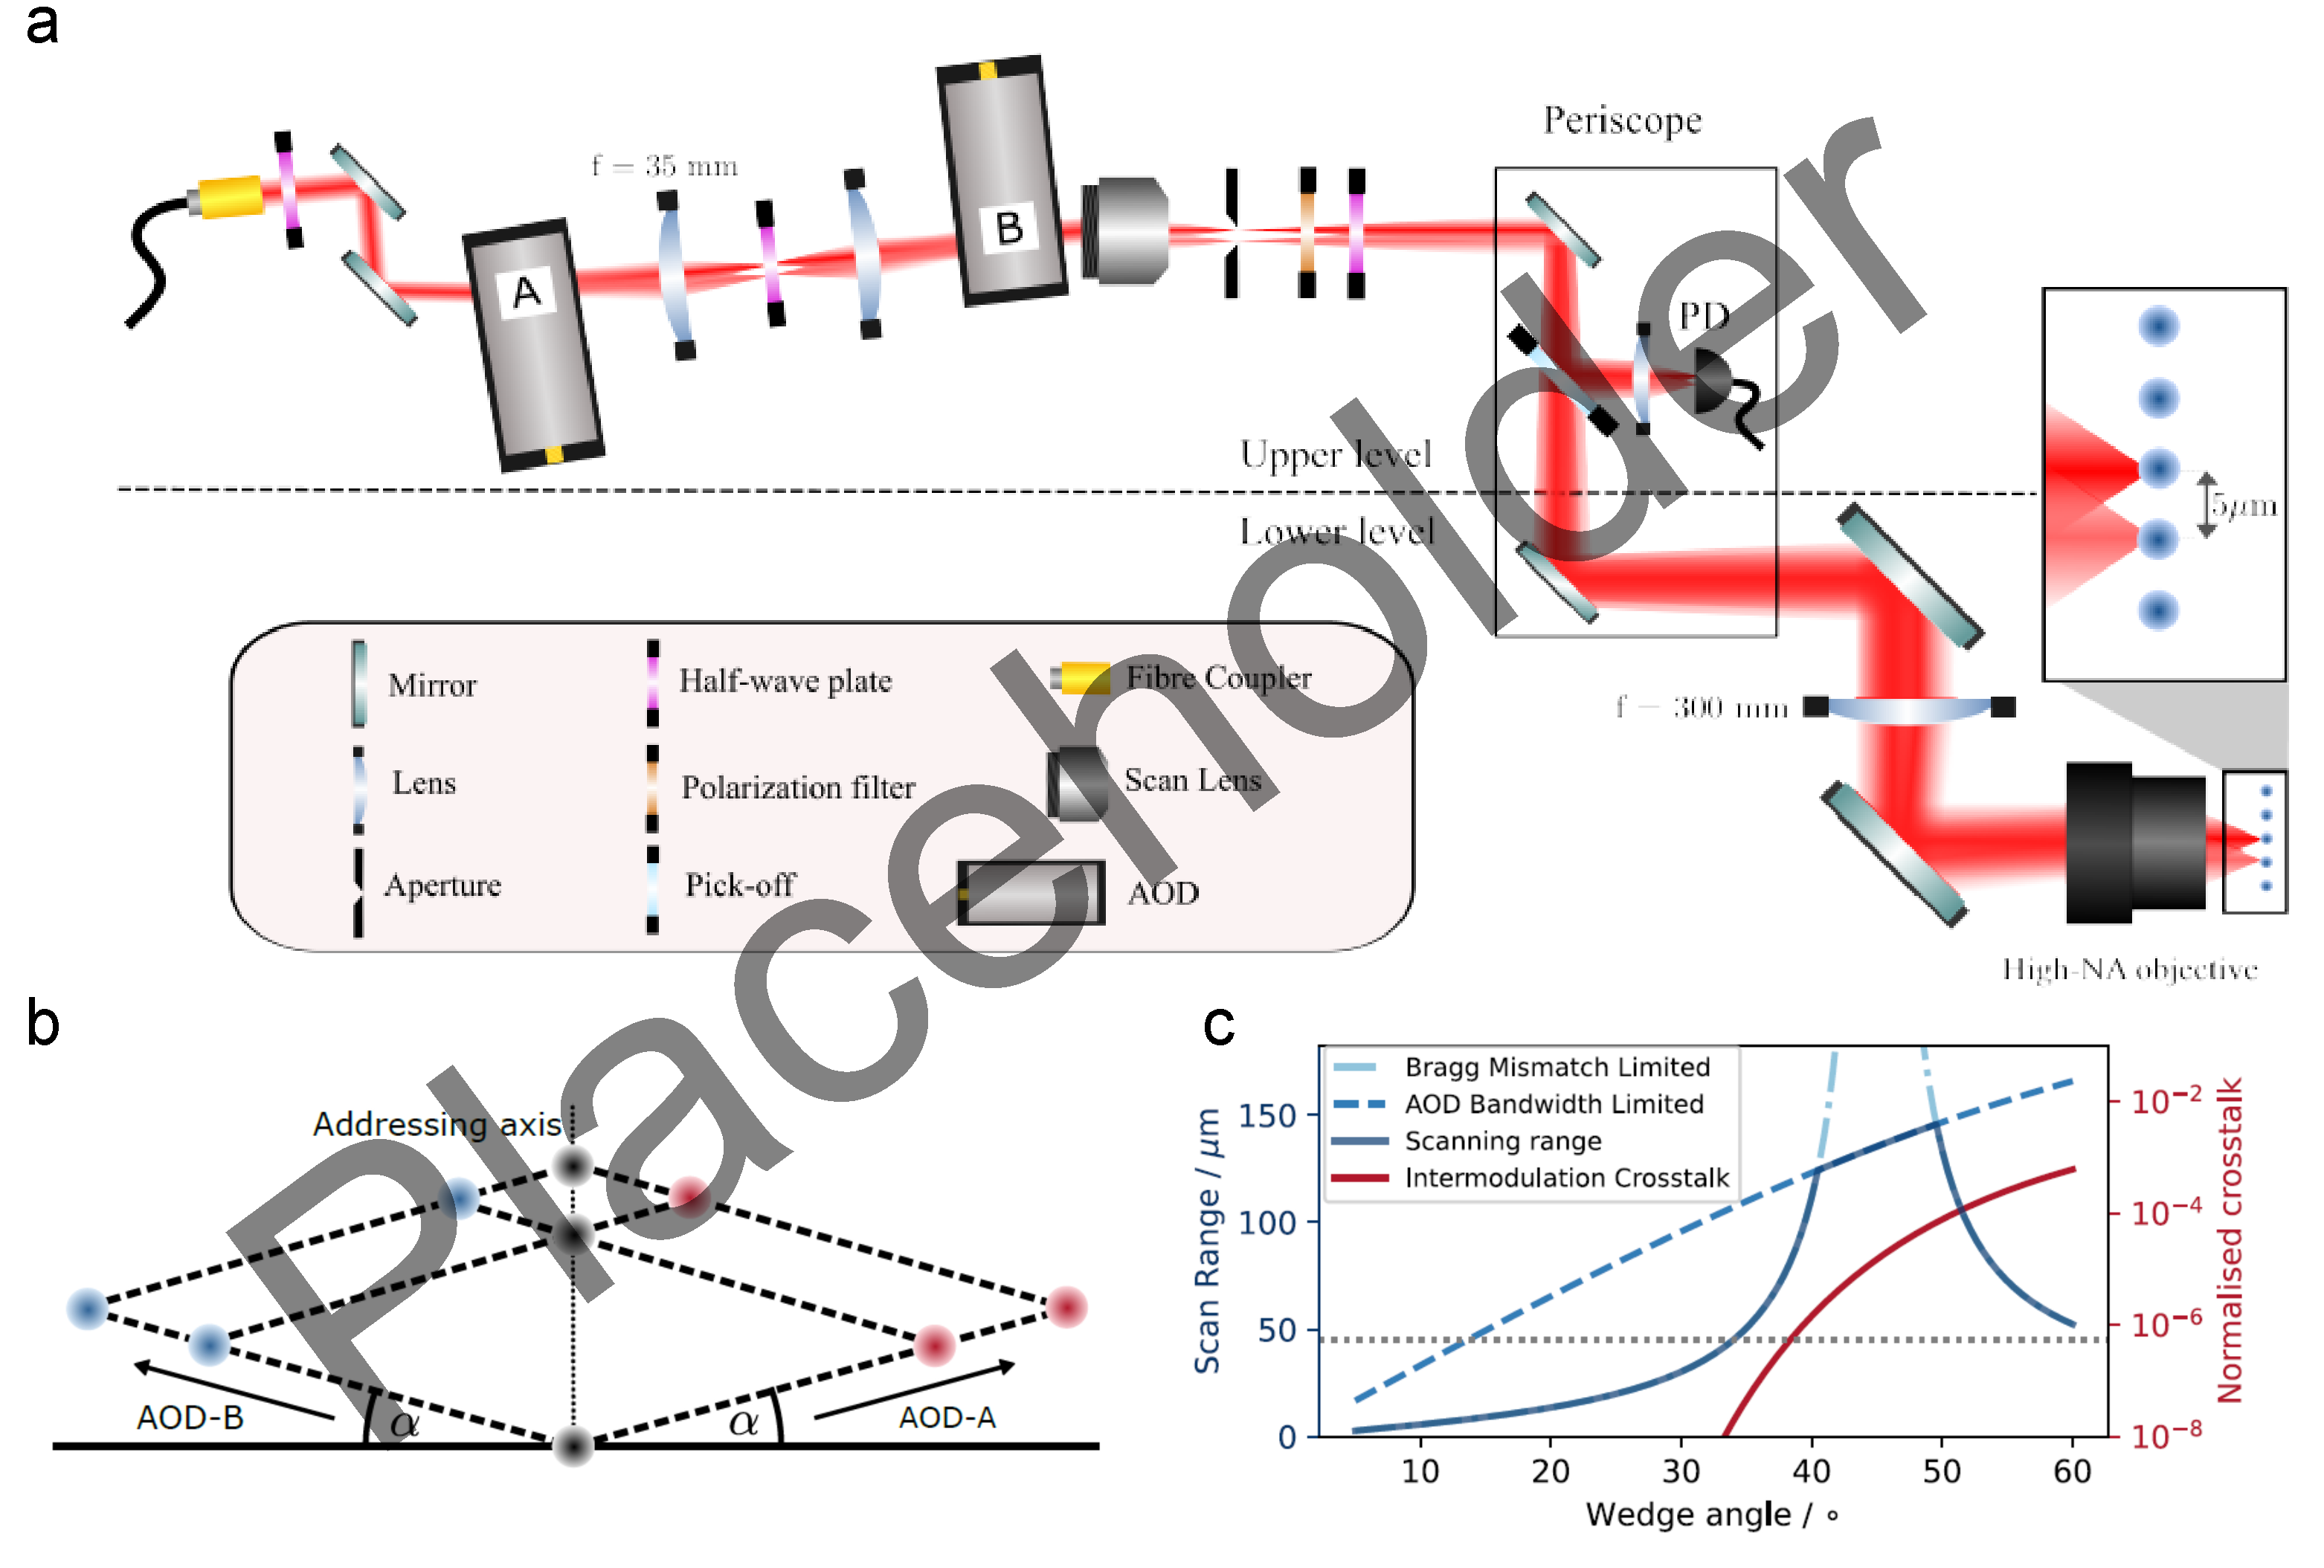
\includegraphics[width=\linewidth]{figures/pdf_figure/ch2/AOD_setup.pdf
        }
    \end{center}
    \caption{
        \todo{Calibrating stark shifts}
        }
    \label{fig:AOD}
\end{figure}
\begin{figure}
    \begin{center}
    \noindent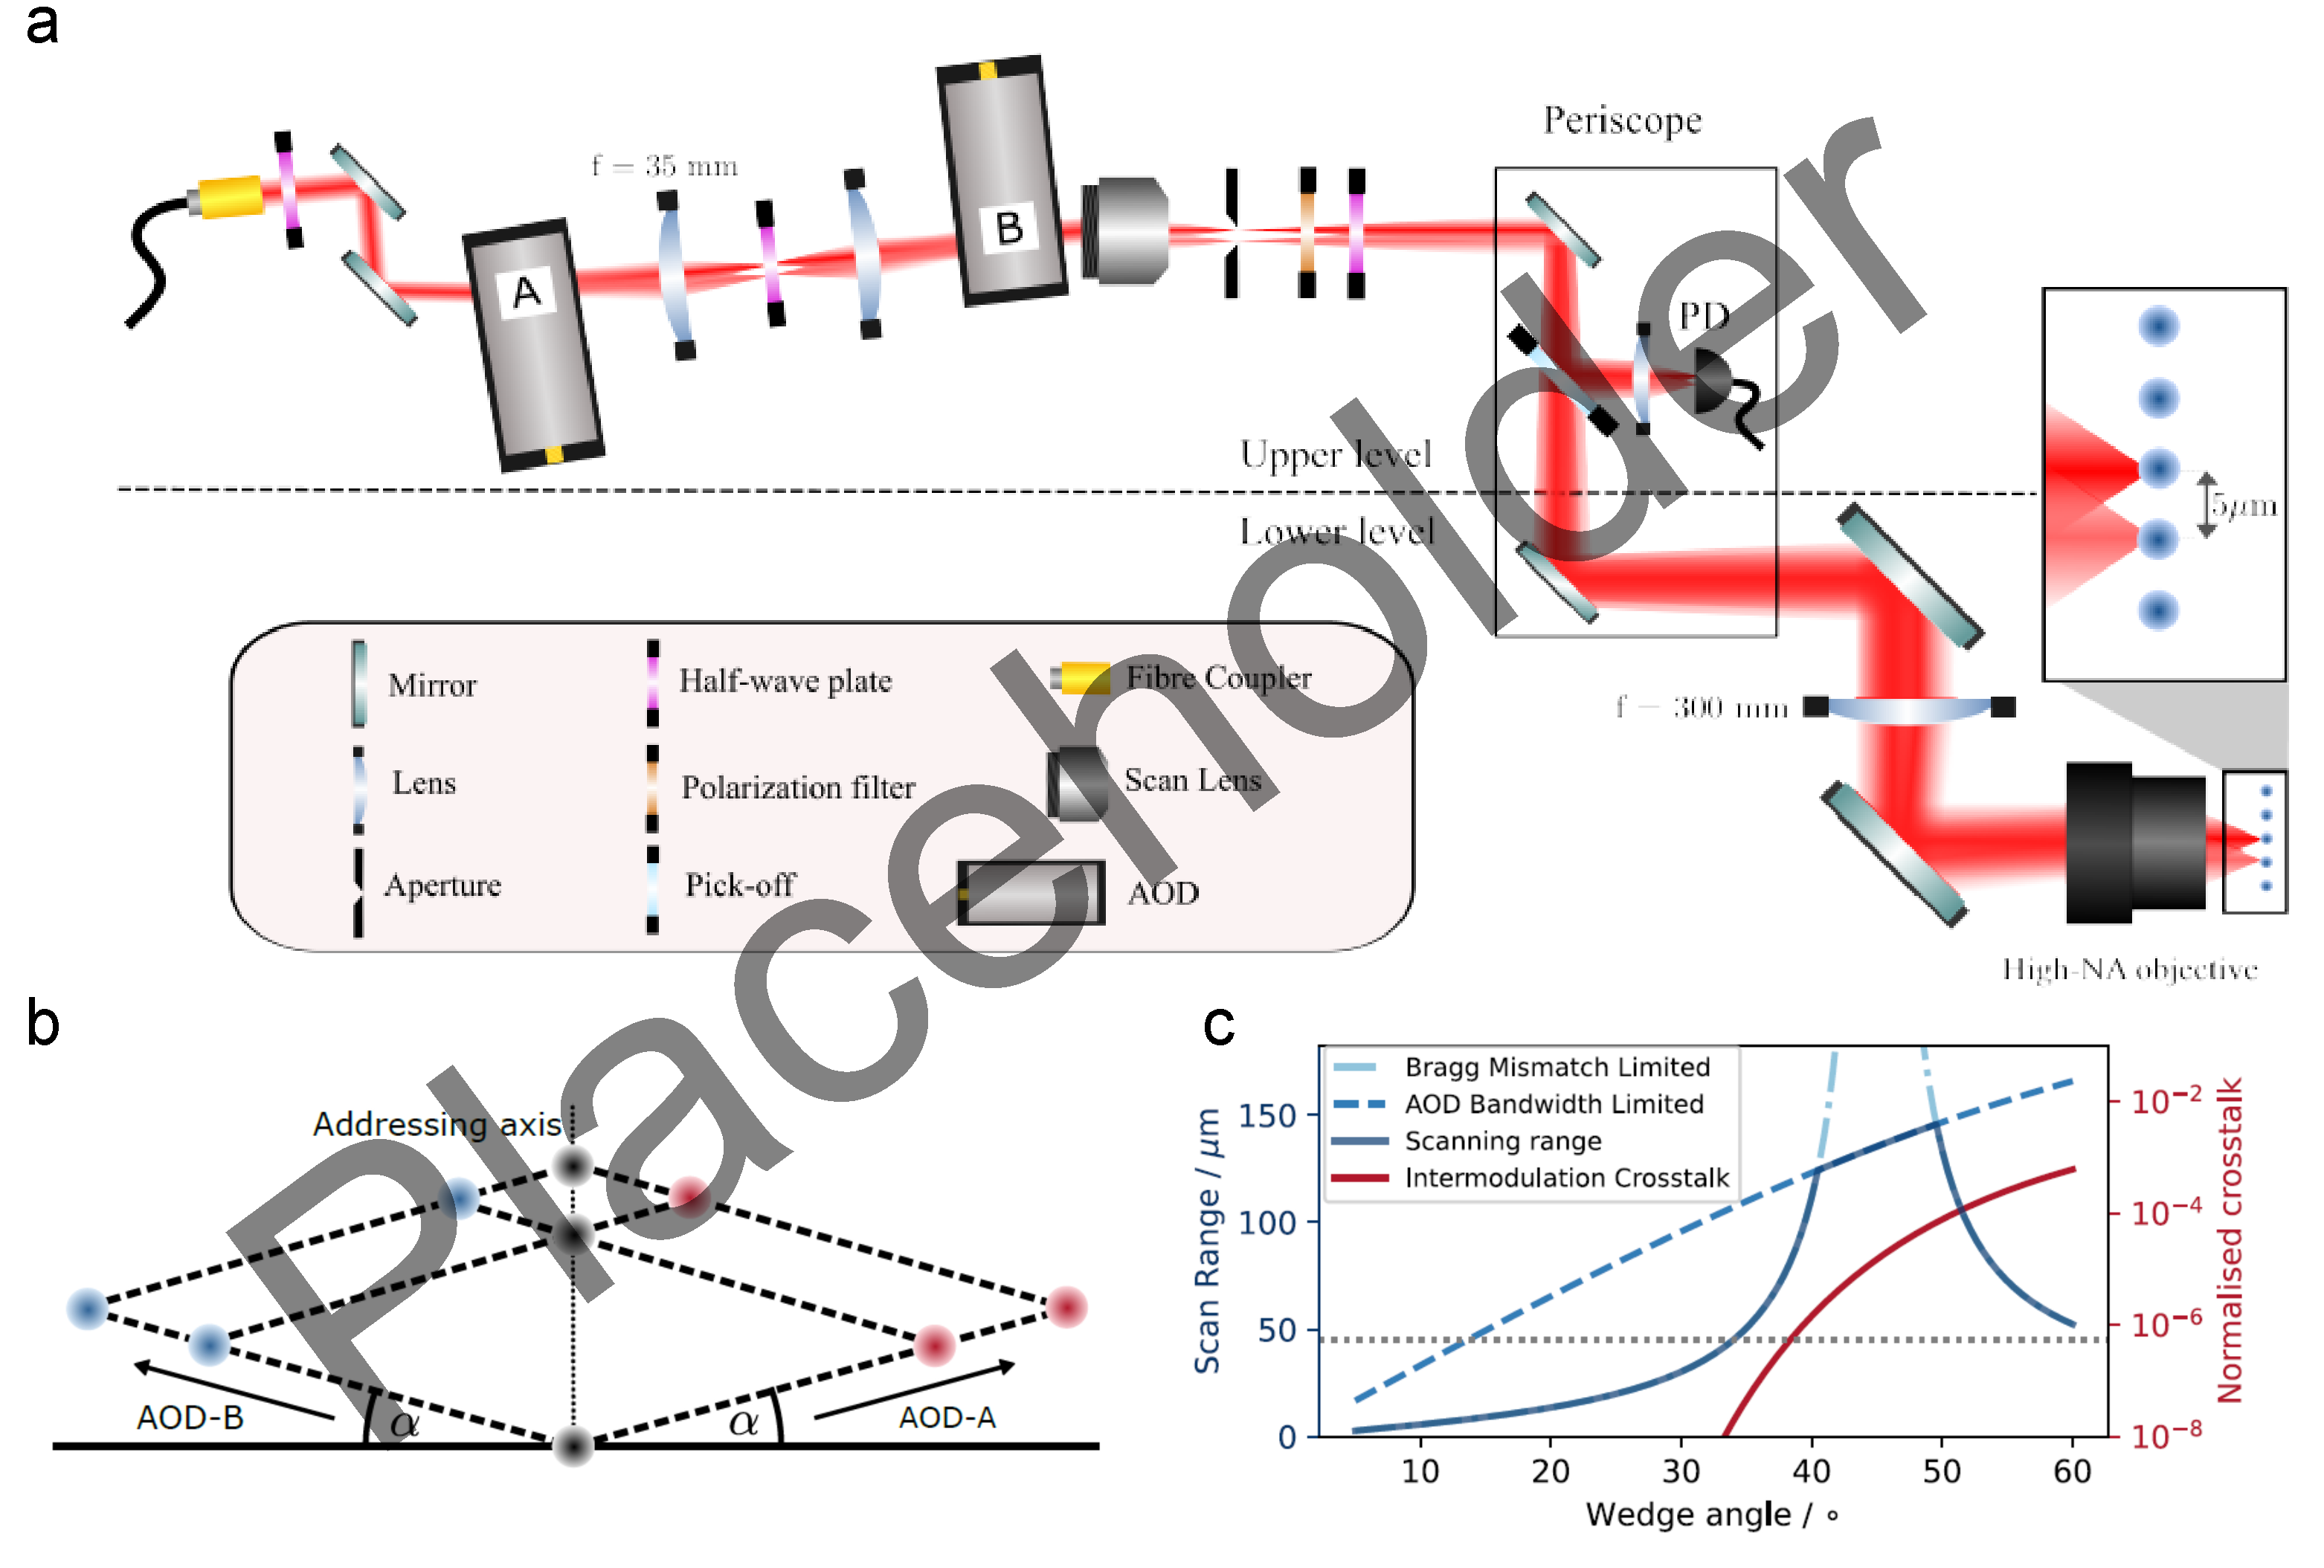
\includegraphics[width=\linewidth]{figures/pdf_figure/ch2/AOD_setup.pdf
        }
    \end{center}
    \caption{
        \todo{Stark shift supplemental figure.}
        }
    \label{fig:AOD}
\end{figure}

\subsection{Scaling to a multi-ion register}
\label{sec:scaling}

\begin{figure}
    \begin{center}
    \noindent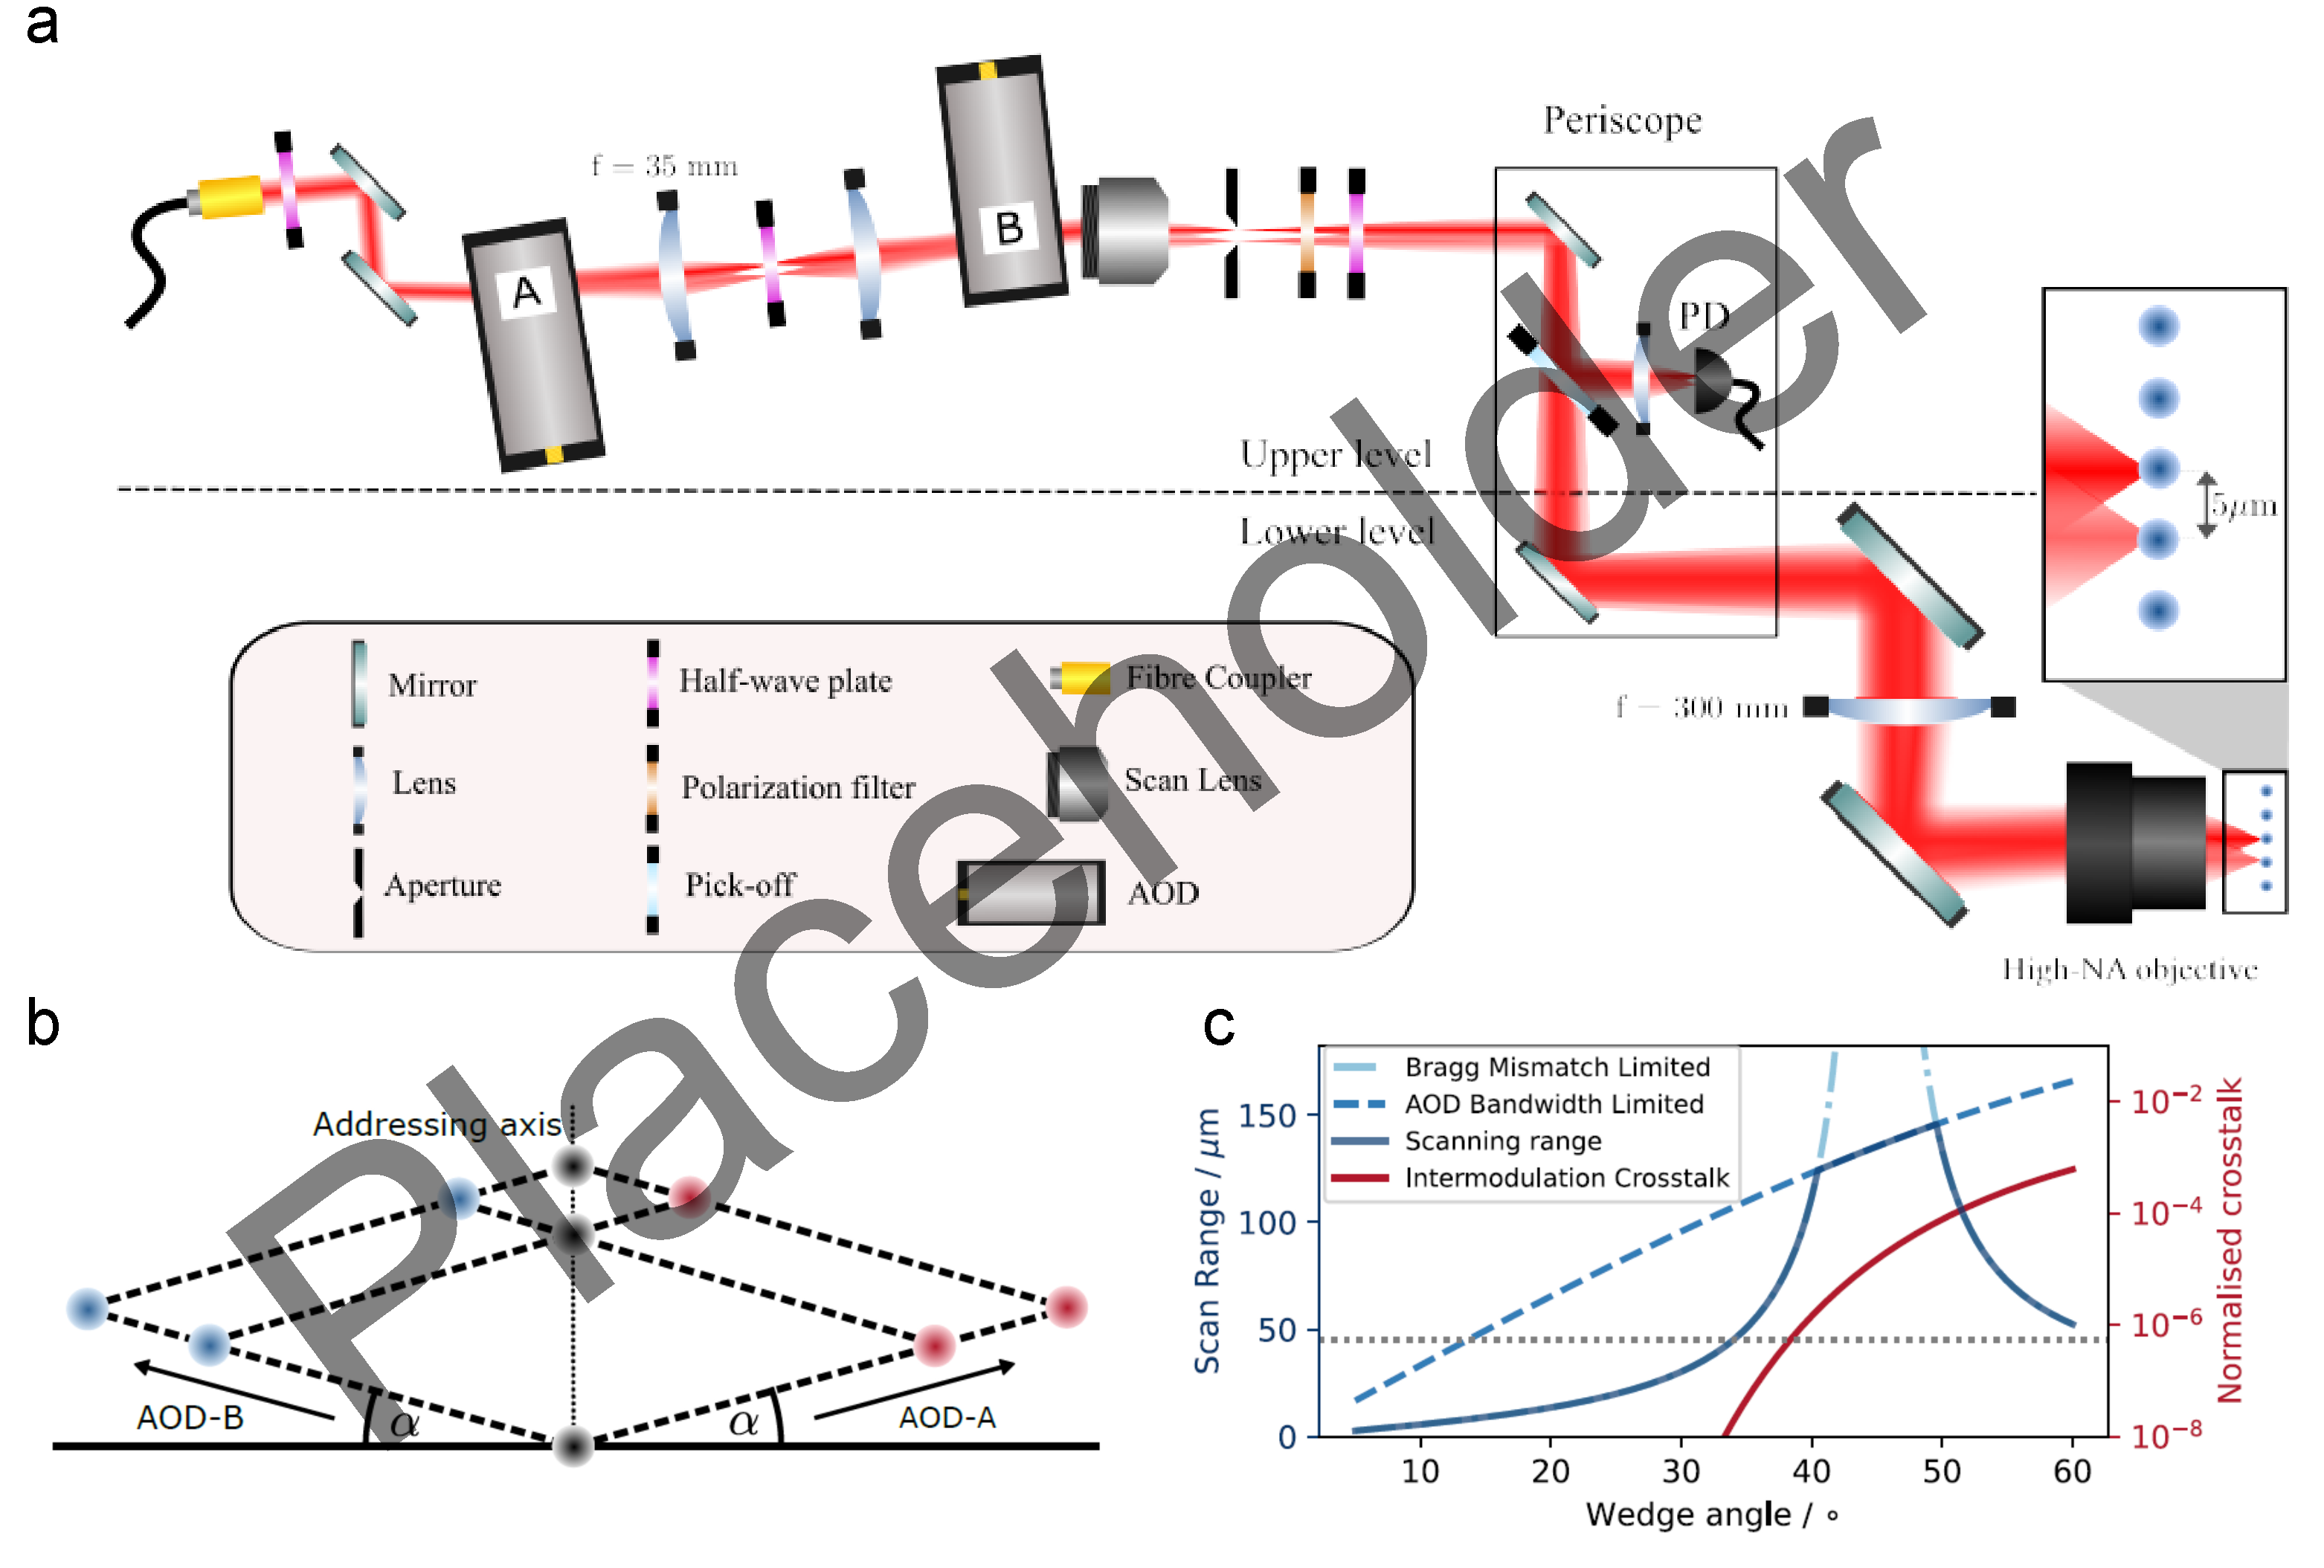
\includegraphics[width=\linewidth]{figures/pdf_figure/ch2/AOD_setup.pdf
        }
    \end{center}
    \caption{
        \todo{Calibrating global beam}
        }
    \label{fig:AOD}
\end{figure}
\begin{figure}
    \begin{center}
    \noindent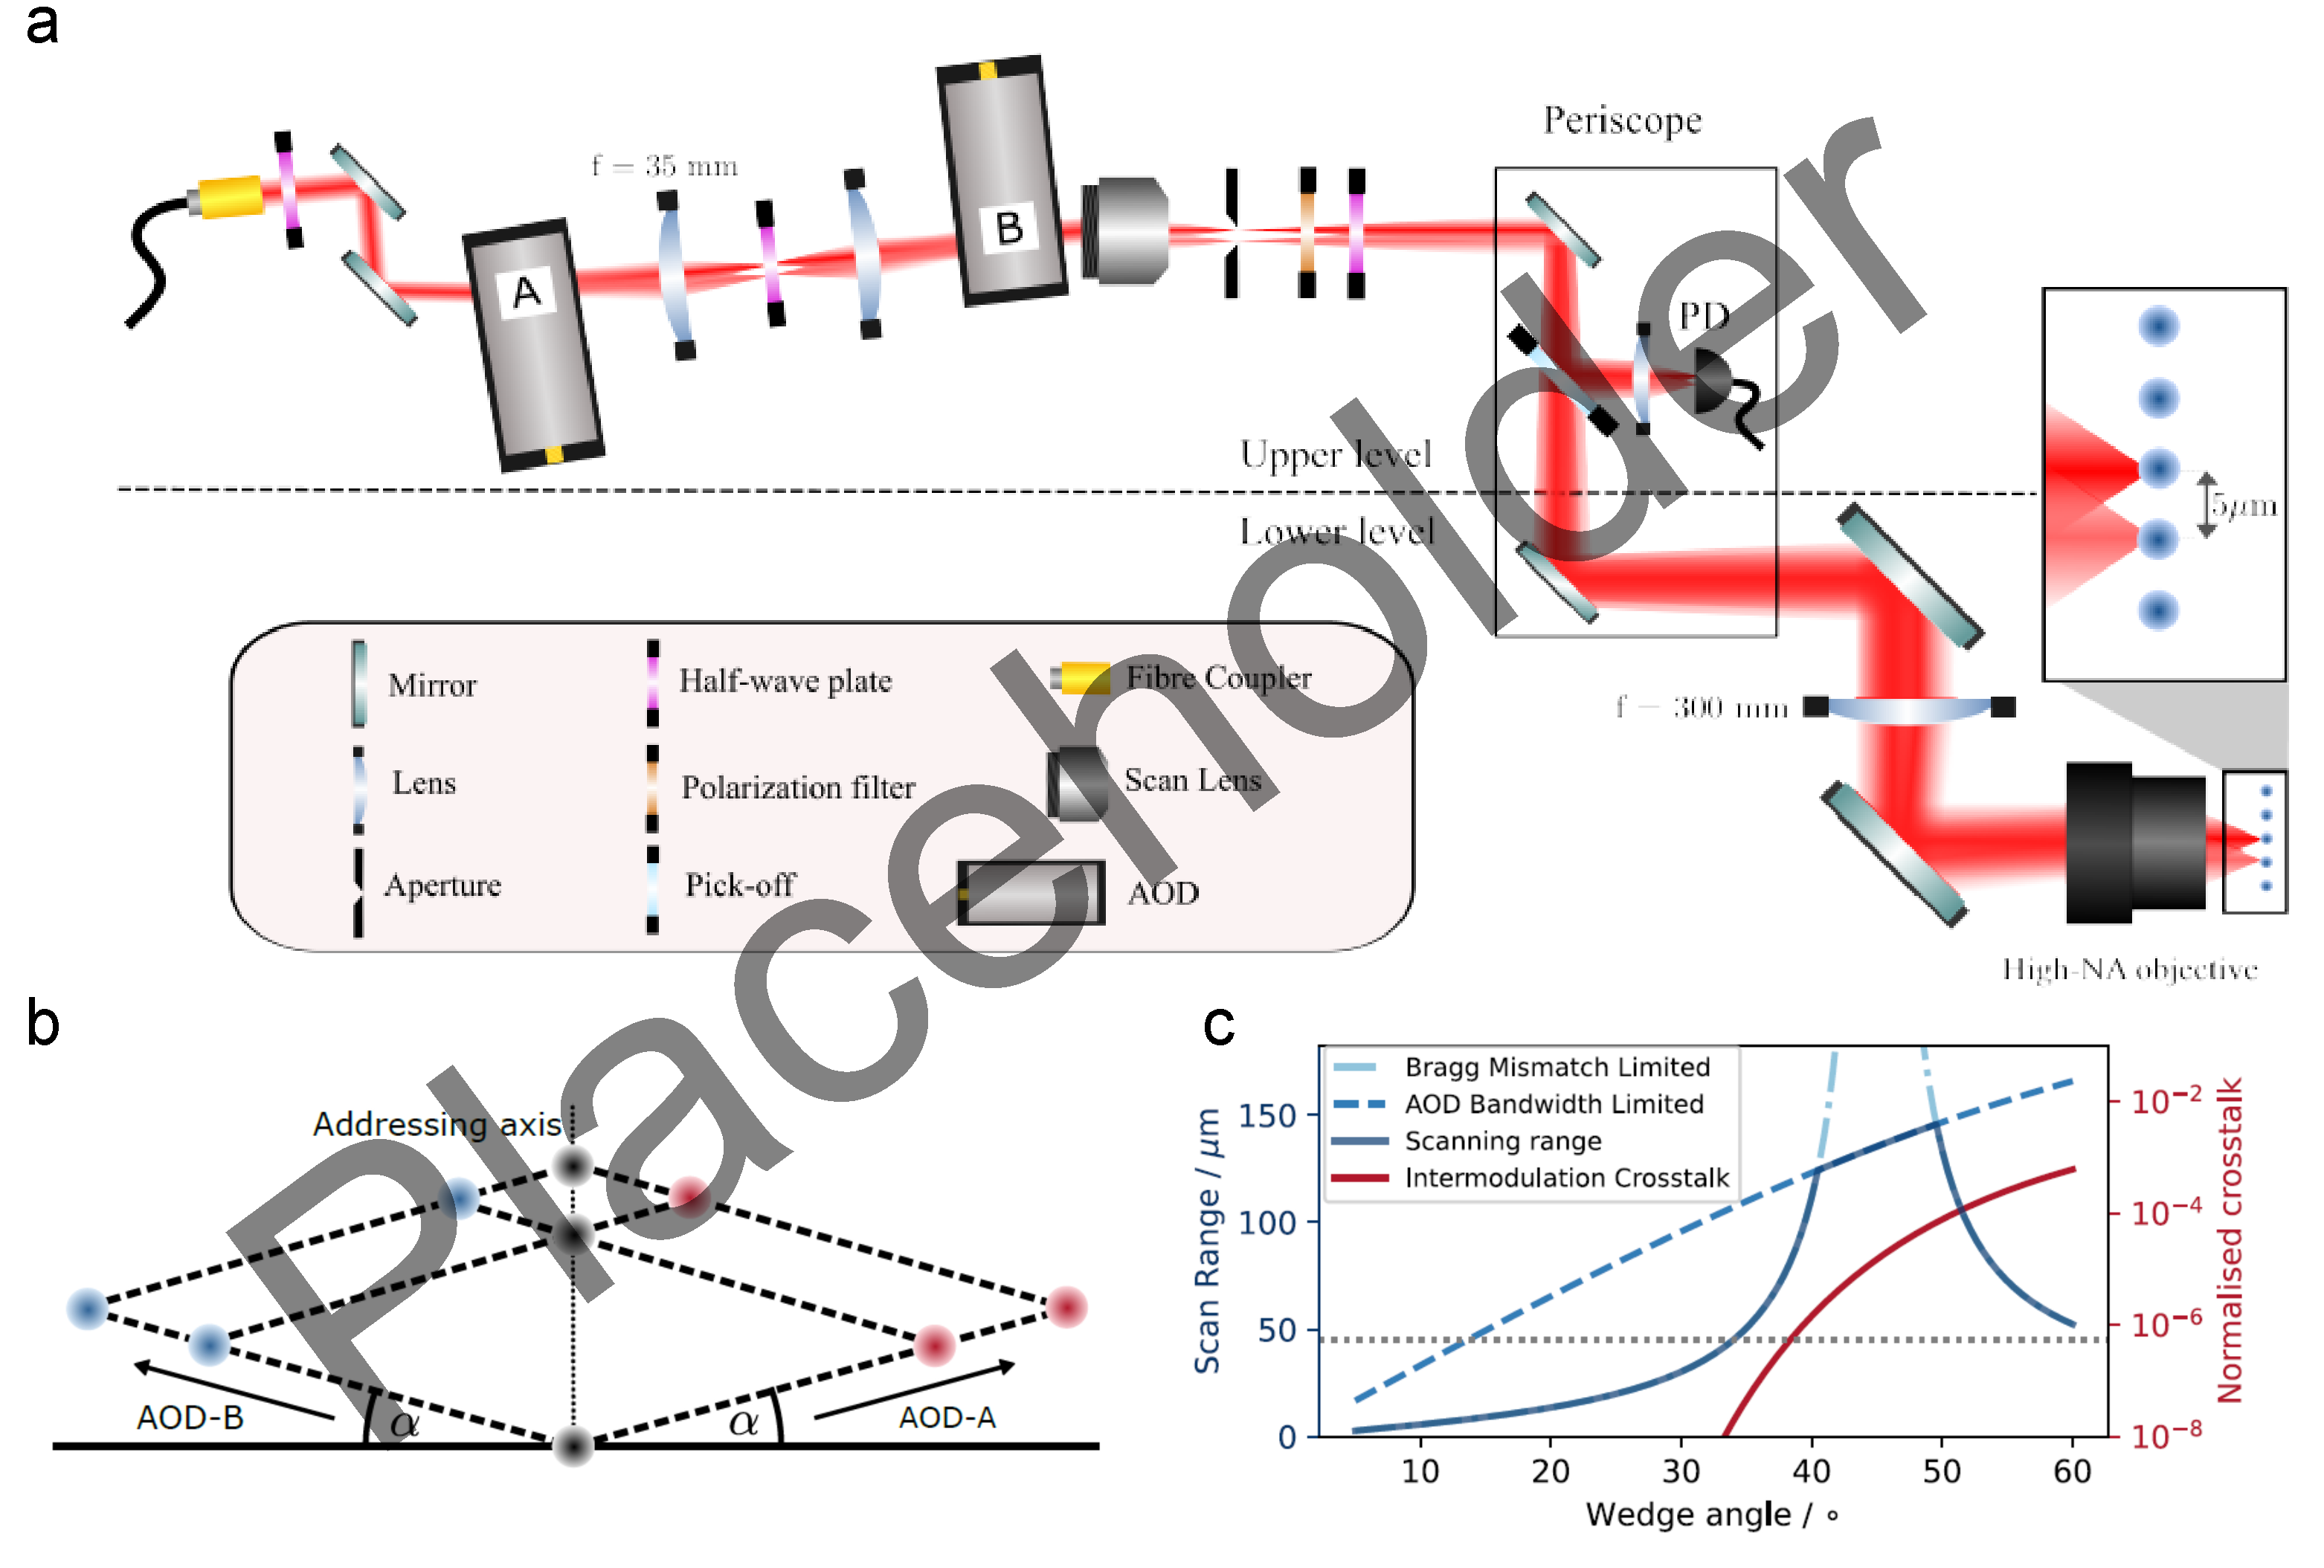
\includegraphics[width=\linewidth]{figures/pdf_figure/ch2/AOD_setup.pdf
        }
    \end{center}
    \caption{
        \todo{Figure 4 from paper.}
        }
    \label{fig:AOD}
\end{figure}

Pairwise $k$-copy RB extends simply to $>2$ qubits: correlated populations
are fit to Eq.~\eqref{eqn:decay} independently for each qubit pair. This
provides a practical diagnostic of pairwise spatial correlations across a
large register, though it does not uniquely determine higher-order
($\geq 3$-body) correlated error terms (see Outlook,
Section~\ref{sec:outlook}). For a register of $k$ qubits, all $k(k-1)/2$
pairwise outcomes are extracted from the same shot record --- no additional
trials on the quantum register are required, though classical
post-processing scales with the number of pair combinations. The protocol
itself requires only synchronised application of identical single-qubit
Clifford sequences and spatially resolved readout.

\todo{(a) Extracted pairwise correlated error
$\varepsilon_{\mathrm{corr}}^{(i,j)}$ for all ion pairs in an 8-ion chain.
(b) Sum of local depolarising errors $(\varepsilon_L+\varepsilon_R)^{(i,j)}$.
(c) Ratio of excess correlated noise to local errors.}{Correlated and local
error per Clifford measured for all qubit pairs in an 8-ion chain (adapted
from manuscript Fig.~4). \todo{Redraw for thesis.}}

This scaling is demonstrated on an eight-ion chain, with parallel
single-qubit rotations driven by an elliptical \SI{729}{\nano\meter} beam of
major-axis waist radius $\SI{52(3)}{\micro\meter}$ aligned to the ion
chain. Addressing multiple qubits in parallel with a single shared drive is
common to both ion-trap and neutral-atom platforms owing to its
experimental simplicity, but unequal illumination across the register leads
to position-dependent over- and under-rotation errors. With axial
confinement of \SI{0.5}{\mega\hertz}, the chain extent is
\SI{35}{\micro\meter}, giving an expected Rabi-frequency difference of
$11(1)\%$ between the outer and inner ions (single-qubit gates were
optimised for the inner ions, $i=4$). The extracted pairwise correlations
show the resulting spatially dependent error structure: both neighbouring
and distant outer-ion pairs exhibit large correlated errors, and in
particular the maximally separated ions $i=1$ and $j=8$ experience similar
under-rotations, producing a strong correlated error despite their spatial
separation.

To improve sensitivity to both correlated and local contributions
simultaneously, a common error offset was intentionally added by randomising
the phase of each implemented $R_x(\pi/2)$ pulse (drawn from a normal
distribution with standard deviation $s_\phi = \SI{0.19}{\radian}$,
producing $\varepsilon_{\mathrm{corr}}^{(0)}=0.025$). This separates the
relevant exponential decay rates and improves the stability of the
correlated-population fits.

\todo{Add the noise-injection methodology in more detail here, including
the complementary Stark-shift-beam injection experiments from the
manuscript SM (App.~``Noise injection methods'', Fig.~S2): two addressing
configurations (correlated two-spot vs.\ independent single-spot Stark
shifts) used to independently calibrate and validate the
$\varepsilon_{\mathrm{corr}}$ vs.\ $\varepsilon_L,\varepsilon_R$ separation
against a known injected error rate.}

% ==========================================================================
\section{Conclusions and outlook}
\label{sec:outlook}

$k$-copy RB efficiently discerns correlated and uncorrelated error channels
acting on a multi-qubit system. Because of the symmetry enforced by
twirling over the diagonal Clifford representation $Cl^{\otimes k}$
(Section~\ref{sec:two_copy_cliff}), structured errors drive the decay of
correlated populations into invariant subspaces in a way that is directly
observable without full process reconstruction. Given a specified error
model, these correlated decays can be used to directly quantify the
magnitude of the individual error channels contributing to the total error
per Clifford.

This method has been proposed and experimentally demonstrated, and its
application extended to an eight-qubit register through pairwise
comparisons (Section~\ref{sec:scaling}). This approach permits highly
efficient parallel data collection: the time required on the device is
independent of qubit number, and the protocol requires exclusively local
operations followed by classical post-processing of correlated survival
rates.

\todo{Expand this Outlook section substantially for the thesis, drawing
together the forward-looking threads seeded earlier in this chapter and in
Chapter~\ref{chap:background}:
\begin{itemize}
    \item Extension to genuine $\geq 3$-body correlated error terms, beyond
    the pairwise diagnostic of Section~\ref{sec:scaling}.
    \item Experimental characterisation of $ZZ$-type entangling errors
    (Section~\ref{sec:noise_models}), not demonstrated here.
    \item Sample-cost / Fisher-information analysis for multi-exponential
    fitting --- flagged as an open numerics question in the manuscript SM
    and not yet resolved.
    \item Non-Markovian (temporally correlated) noise, via repeated
    identical Clifford RB sequences applied at different times on a single
    qubit, exploiting the same correlated-outcome analysis used here for
    spatial correlations.
    \item Character-RB-style initial-state engineering
    (Section~\ref{sec:analytic_predictions}) to isolate single exponential
    decays and reduce sample cost.
\end{itemize}
}
